% Use the following line _only_ if you're still using LaTeX 2.09.
%\documentstyle[icml2016,epsf,natbib]{article}
% If you rely on Latex2e packages, like most moden people use this:
\documentclass{article}

% use Times
\usepackage{times}
% For figures
\usepackage{graphicx} % more modern
%\usepackage{epsfig} % less modern
\usepackage{subfigure} 

% For citations
\usepackage{natbib}
\usepackage{bm}

% For algorithms
\usepackage{algorithm}
\usepackage{color}
\usepackage{pbox}

\usepackage{algorithmic}
% As of 2011, we use the hyperref package to produce hyperlinks in the
% resulting PDF.  If this breaks your system, please commend out the
% following usepackage line and replace \usepackage{icml2016} with
% \usepackage[nohyperref]{icml2016} above.
\usepackage{hyperref}
% Packages hyperref and algorithmic misbehave sometimes.  We can fix
% this with the following command.
\newcommand{\theHalgorithm}{\arabic{algorithm}}
% Employ the following version of the ``usepackage'' statement for
% submitting the draft version of the paper for review.  This will set
% the note in the first column to ``Under review.  Do not distribute.''
\usepackage[accepted]{icml2016} 

% Employ this version of the ``usepackage'' statement after the paper has
% been accepted, when creating the final version.  This will set the
% note in the first column to ``Proceedings of the...''
%\usepackage[accepted]{icml2016}









%%%%%%%%%%%%%%%%%%%%%%%%%%%%%%%%%%%%%%%%%%%%%%%%%%%%%%%%%%%%%%%%%%%%%%%%%%

\usepackage{url} 
\usepackage{bm}
\usepackage{bbm}
\usepackage{amsmath,amssymb}
\usepackage{xspace}
\usepackage{bm} 
\usepackage{dsfont}
\usepackage{psfrag}
\usepackage{rotating}
\usepackage{epstopdf}
\usepackage{booktabs}

\floatstyle{ruled}
\newfloat{algo}{thp}{lop} 
\floatname{algo}{Algorithm}
 
\newcommand{\bydef}{{\displaystyle\mathop{=}^{\textrm{def}}}}
\newcommand{\softmax}{\mathop{\varsigma}}
\newcommand{\OmegaSpace}{\Omega}
\renewcommand{\O}{\mathcal{O}}
\newcommand{\Yspace}{\mathcal{Y}}
\newcommand{\Xspace}{\mathcal{X}}
\newcommand{\Zspace}{\mathcal{Z}}
\newcommand{\Bspace}{\mathcal{B}}
\newcommand{\TauSpace}{\mathcal{T}}
\newcommand{\f}{f}
\newcommand{\g}{g}
\newcommand{\h}{h}
\newcommand{\z}{z}
\newcommand{\p}{p}
\newcommand{\q}{q}
\newcommand{\entropy}{\mathcal{H}}
\newcommand{\jaak}{\lambda}
\newcommand{\trace}{\mathop{\textrm{tr}}}
\newcommand{\diag}{\mathop{\textrm{diag}}}
\newcommand{\lambdavec}{\bm{\lambda}}

\renewcommand{\a}{a}
\renewcommand{\b}{b}
\renewcommand{\d}{d}
\newcommand{\w}{w}
\renewcommand{\t}{t}
\newcommand{\x}{x}
\newcommand{\y}{y}
%\newcommand{\z}{z}
\renewcommand{\S}{\mathcal{S}}
\newcommand{\F}{\mathcal{F}}
\newcommand{\normdist}{\mathcal{N}}
\newcommand{\poissdist}{\mathcal{P}}
\newcommand{\s}{s}
%\renewcommand{\L}{\Lambda}

\newcommand{\transp}{^{T}}
\newcommand{\tendsto}{\longrightarrow}
\newcommand{\one}{\bm{1}}
\newcommand{\dist}{\mathcal{L}}
\newcommand{\proba}{P}
\newcommand{\grad}{\nabla}

\newcommand{\A}{\bm{A}}
\newcommand{\D}{\bm{D}}
\newcommand{\U}{\bm{U}}
\newcommand{\V}{\bm{V}}
\renewcommand{\P}{P}
\newcommand{\Q}{Q}
\newcommand{\I}{\bm{I}}
\newcommand{\zeros}{\bm{0}}
\newcommand{\X}{\bm{X}}
\newcommand{\Y}{\bm{Y}}
\newcommand{\W}{\bm{W}}
\newcommand{\sumop}{\mathrm{sum}}


\newcommand{\Expectation}[2]{\mathbb{E}_{#1}\left[#2\right]}
\newcommand{\Expectationsmall}[2]{\mathbb{E}_{#1}[#2]}
\newcommand{\Var}[2]{\textnormal{Var}_{#1}\left[#2\right]}
\newcommand{\Varsmall}[2]{\textnormal{Var}_{#1}(#2)}
\newcommand{\Indicsmall}[1]{\textrm{I}_{\left\lbrace#1\right\rbrace}}
\newcommand{\Indic}[1]{\textrm{I}\left\lbrace#1\right\rbrace}
\newcommand{\pen}{\textrm{pen}}


\newcommand{\complexSpace}{\mathbb{C}}
\renewcommand{\Re}{\mathbb{R}}
\newcommand{\C}{\complexSpace} %Complex space
\newcommand{\R}{\Re} %Real space
\newcommand{\real}{\mathrm{Re}}
\newcommand{\imag}{\mathrm{Im}}
%\def\bin{\bar}
\newcommand{\randn}{\mathrm{randn}}
\newcommand{\srank}{\mathrm{rank}_{\pm}}
\newcommand{\lrank}{\mathrm{rank}}
\newcommand{\sign}{\mathrm{sign}}

%\newenvironment{proof}{\textbf{Proof~}\small}{\hfill$\Box$\\}

\providecommand{\U}[1]{\protect\rule{.1in}{.1in}}
%EndMSIPreambleData
\newcommand{\be}{\begin{equation}}
\newcommand{\ee}{\end{equation}}
\newcommand{\bd}{\begin{definition}}
\newcommand{\ed}{\end{definition}}
\newcommand{\ba}{\begin{algorithm}}
\newcommand{\ea}{\end{algorithm}}
\newcommand{\br}{\begin{problem}}
\newcommand{\er}{\end{problem}}
\newcommand{\bex}{\begin{example}}
\newcommand{\eex}{\end{example}}
\newcommand{\bt}{\begin{theorem}}
\newcommand{\et}{\end{theorem}}
\newcommand{\BFAT}{\mbox{\bf B}}
\newcommand{\EFAT}{\mbox{\bf E}}
\newcommand{\PFAT}{\mbox{\bf P}}
\newcommand{\la}[1]{\label{#1}}
\newcommand{\re}[1]{(\ref{#1})}
\newtheorem{theorem}{Theorem}
\newtheorem{acknowledgement}[theorem]{Acknowledgement}
%\newtheorem{algorithm}[theorem]{Algorithm}
\newtheorem{axiom}[theorem]{Axiom}
\newtheorem{case}[theorem]{Case}
\newtheorem{claim}[theorem]{Claim}
\newtheorem{conclusion}[theorem]{Conclusion}
\newtheorem{condition}[theorem]{Condition}
\newtheorem{conjecture}[theorem]{Conjecture}
\newtheorem{corollary}[theorem]{Corollary}
\newtheorem{criterion}[theorem]{Criterion}
\newtheorem{definition}[theorem]{Definition}
\newtheorem{example}[theorem]{Example}
\newtheorem{exercise}[theorem]{Exercise}
\newtheorem{lemma}[theorem]{Lemma}
\newtheorem{notation}[theorem]{Notation}
\newtheorem{problem}[theorem]{Problem}
\newtheorem{proposition}[theorem]{Proposition}
\newtheorem{remark}[theorem]{Remark}
\newtheorem{solution}[theorem]{Solution}
\newtheorem{summary}[theorem]{Summary}
\newenvironment{proof}[1][Proof]{\noindent\textbf{#1.} }{\ \rule{0.5em}{0.5em}}
\newcommand{\Tr}{Trace}
\newcommand{\identity}{I}

\newcommand{\fix}{\marginpar{FIX}}
\newcommand{\new}{\marginpar{NEW}}

\def\ifa{\iffalse}
\def\ifappendix{\iftrue}

% command to highlight comments
\newcommand{\mynote}[2]{{\bf \color{red}{#1}:~{#2}}}


\newcommand{\Relation}{\mathbf{X}}
\newcommand{\ObsTensor}{\mathbf{Y}}
\newcommand{\EntitySpace}{\mathcal{E}}
\newcommand{\RelationSpace}{\mathcal{R}}
\newcommand{\score}{s}



%%%%%%%%%%%%%%%%%%%%%%%%%%%%%%%%%%%%%%%%%%%%%%%%%%%%%%%%%%%%%%%%%%%%%%%%%%%%%%%%
%Notations for KB factorization stuff, following Nickel notations (Review paper)

\newcommand{\Ne}{N_e} %Number of entities
\newcommand{\Nr}{N_r} %Number of relations
\newcommand{\Nd}{N_d} %Number of training examples
\newcommand{\rank}{K} %Set of positive examples
\newcommand{\setpos}{\mathcal{D^+}} %Set of positive examples
\newcommand{\setneg}{\mathcal{D^-}} %Set of positive examples
\newcommand{\paramspace}{\Theta} %Set of parameters
\newcommand{\sample}{x_{s,r,o}}  %sample
\newcommand{\sampval}{y_{s,r,o}}  %sample
\newcommand{\setent}{\mathcal{E}} %Set of entities
\newcommand{\setrel}{\mathcal{R}} %Set of relations
\newcommand{\eemb}{e} %entity vector
\newcommand{\Eemb}{E} %Entity matrix
\newcommand{\remb}{\mathbf{r}} %relation vector
\newcommand{\Remb}{\mathbf{R}} %Relation matrix
\newcommand{\wemb}{w} %relation vector
\newcommand{\Wemb}{W} %Relation matrix
\renewcommand{\j}{\mathbf{j}}

\def\tt{\texttt}

\usepackage[textsize=tiny]{todonotes}
%\usepackage[disable,textsize=small]{todonotes} %removes the todo notes
\newcommand{\Johans}[1]{\todo[inline,backgroundcolor=green!20!green]{Johans: #1}}

\newcommand{\G}[1]{\todo[inline,backgroundcolor=green!20!red]{Gui: #1}}

\newcommand{\Seb}[1]{\todo[inline,backgroundcolor=white!20!white]{Seb: #1}}

\newcommand{\Eric}[1]{\todo[inline,backgroundcolor=blue!20!white]{Eric: #1}}
%%%%%%
\newcommand{\TT}[1]{\todo[inline,backgroundcolor=violet!50!white]{Th\'eo: #1}}

%\graphicspath{{figures/}}


% The \icmltitle you define below is probably too long as a header.
% Therefore, a short form for the running title is supplied here:
\icmltitlerunning{Complex Embeddings for Simple Link Prediction}

\begin{document} 

\twocolumn[
\icmltitle{Complex Embeddings for Simple Link Prediction}
%\icmltitle{Complex Embeddings for Simple Link Prediction}

% It is OKAY to include author information, even for blind
% submissions: the style file will automatically remove it for you
% unless you've provided the [accepted] option to the icml2016
% package.
\icmlauthor{Th\'eo Trouillon$^{1,2}$}{theo.trouillon@xrce.xerox.com}
\icmlauthor{Johannes Welbl$^{3}$}{j.welbl@cs.ucl.ac.uk}
\icmlauthor{Sebastian Riedel$^{3}$}{s.riedel@cs.ucl.ac.uk}
\icmlauthor{\'Eric Gaussier$^{2}$}{eric.gaussier@imag.fr}
\icmlauthor{Guillaume Bouchard$^{3}$}{g.bouchard@cs.ucl.ac.uk}
\icmladdress{$^{1}$ Xerox Research Centre Europe, 6 chemin de Maupertuis, 38240 Meylan, FRANCE\\$^{2}$ Universit\'e Grenoble Alpes, 621 avenue Centrale, 38400 Saint Martin d'H\`eres, FRANCE\\$^{3}$ University College London, Gower St, London WC1E 6BT, UNITED KINGDOM}

% You may provide any keywords that you 
% find helpful for describing your paper; these are used to populate 
% the "keywords" metadata in the PDF but will not be shown in the document
\icmlkeywords{embeddings, factorization, knowledge graph, complex numbers, link prediction, statistical relational learning, complex embeddings, }

\todototoc

\vskip 0.3in
]

\begin{abstract} 
In statistical relational learning, the link prediction problem is key to automatically understand the structure of large knowledge bases. As in previous studies, we propose to solve this problem through latent factorization. However, here we make use of complex valued embeddings. The composition of complex embeddings can handle a large variety of binary relations, among them symmetric and antisymmetric relations. Compared to state-of-the-art models such as Neural Tensor Network and Holographic Embeddings, our approach based on \emph{complex} embeddings is arguably \emph{simpler}, as it only uses the Hermitian dot product, the complex counterpart of the standard dot product between real vectors. Our approach is scalable to large datasets as it remains linear in both space and time, while consistently outperforming alternative approaches on standard link prediction benchmarks.\footnote{Code is available at: \url{https://github.com/ttrouill/complex}}
\end{abstract} 









\section{Introduction}

% Driven by the W3C standard data representation for the Semantic Web, the Resource Description Framework (RDF), various Knowledge Bases (KB) have been collaboratively created in recent years
Web-scale knowledge bases (KBs) provide a structured representation of world knowledge, with projects such as DBPedia~\cite{dbpedia}, Freebase~\cite{Bollacker2008} or the Google Knowledge Vault~\cite{Dong:2014:KnowledgeVault}. 
They enable a wide range of applications such as recommender systems, question answering or automated personal agents. The incompleteness of these KBs has stimulated \mbox{research} into predicting missing entries, a task known as link prediction that is one of the main problems in Statistical Relational Learning~\citep[SRL,][]{Getoor2007}.

%A wide range of applications, such as question answering or automated personal agents can draw from KBs and due to their relational nature, KBs are also a perfect fit for Statistical Relational Learning (SRL)~\cite{Getoor2007,nickel_2016_review}. Statistical Relational Learning (SRL)~\cite{Getoor2007,nickel_2016_review}, a growing field in Machine Learning. 

%\Seb{How important is that KBs need to be large? Is Wordnet really large? Could/Should we be more generic?}

% Modelling arbitrary relational knowledge 
% structures is today a growing field in Machine Learning, known as

KBs express data as a directed graph with labeled edges (relations) between nodes (entities). Natural redundancies among the recorded relations often make it possible to fill in the missing entries of a KB. 
%In large KBs many facts are missing, but there often are natural redundancies 
%among the recorded relations. These redundancies can be exploited to fill in missing entries 
%of the KB or for de-noising the database.
As an example, the relation \tt{CountryOfBirth} is not recorded for all entities, 
but it can easily be inferred if the relation \tt{CityOfBirth} is known. 
The goal of link prediction is the automatic discovery of such regularities. However, many relations are non-deterministic:  the combination of the two facts \tt{IsBornIn(John,Athens)} and \tt{IsLocatedIn(Athens,Greece)} does not always imply the fact \tt{HasNationality(John,Greece)}. 
%Integrating other contextual information however can lead to much better predictions.
%Hence it is required to handle all the other facts about these relations (\tt{IsBornIn}, \tt{IsLocatedIn} and \tt{HasNationality}) and entities (\tt{John, Athens} and \tt{Greece}) in a probabilistic fashion. % is required to leverage good predictions. 
Hence, it is required to handle other facts involving these relations or entities in a probabilistic fashion.

To do so, an increasingly popular method is to state the link prediction task as a 3D binary tensor completion problem, where each slice is the adjacency matrix of one relation type in the knowledge graph.
%\paragraph{Low-rank factorization}
%Low-rank models, also called latent vector models or embedding models, have been studied by several authors who have shown that they lead to scalable, simple and accurate algorithms. 
%\Johans{scalable == linear? simple == simple composition function? accurate == yielding accurate predictions?}
Completion based on low-rank factorization or \emph{embeddings} has been popularized with the Netflix challenge \cite{koren_netflix}. A partially observed matrix or tensor is decomposed into a product of embedding matrices with much smaller rank, resulting in fixed-dimensional vector representations %, often called embeddings, 
for each entity and relation in the database. 
%The score %$\phi_{\Theta}(s,r,o)$, 
%for a given fact \emph{r(s,o)} (meaning the subject $s$ is linked to object $o$ through relation $r$) can then be recovered as a multi-linear product between the embedding vectors of the entities and relation involved in the fact~\cite{nickel_2016_review}.
For a given fact \emph{r(s,o)} in which subject $s$ is linked to object $o$ through relation $r$, the score can then be recovered as a multi-linear product between the embedding vectors of $s$, $r$ and $o$ ~\cite{nickel_2016_review}.
%Several authors have developed simple and scalable algorithms that employ low-rank factorization techniques for the KB completion task.

%\Seb{citations here?}
%\Johans{I reformulated this bit, the old part is still commented out in the .tex}

% On dashes: http://tex.stackexchange.com/questions/3819/dashes-vs-vs
Binary relations in KBs exhibit various types of patterns: hierarchies and compositions like \tt{FatherOf}, \tt{OlderThan} or \tt{IsPartOf}---with partial/total, strict/non-strict orders---and  equivalence relations like \tt{IsSimilarTo}. As described in \citet{Bordes2013}, a relational model should (a) be able to learn all \mbox{combinations} of these properties, namely reflexivity/irreflexivity, symmetry/antisymmetry and transitivity, and (b) be linear in both time and memory in order to scale to the size of present day KBs, and keep up with their growth. 

Dot products of embeddings scale well and can naturally handle both symmetry and (ir-)reflexivity of relations; using an appropriate loss function even enables transitivity~\cite{bouchard2015}.
%Dot products of embeddings scale well and can naturally handle both symmetry and (i-)reflexivity -- when combined with relation embeddings -- and using an appropriate loss function enables transitivity~\cite{bouchard2015}. 
However, dealing with antisymmetric relations has so far almost always implied an explosion of the number of parameters \cite{Nickel2011,socher2013reasoning} (see Table \ref{tab:scoring}), making models prone to overfitting. Finding the best ratio between expressiveness and parameter space size is the keystone of embedding models.
%with the exception of TransE \citet{bordes2013translating}. Although it is theoretically able to handle antisymmetry, it actually performs poorly in practice (see Section \ref{{sec:expe}}).

In this work we argue that the standard dot product between embeddings can be a very effective composition function, provided that one uses the right \emph{representation}. Instead of using embeddings containing real numbers we discuss and demonstrate the capabilities of complex embeddings. When using complex vectors, i.e. vectors with entries in $\complexSpace$,  the dot product is often called the \emph{Hermitian} (or sesquilinear) dot product, as it involves the conjugate-transpose of one of the two vectors. 
%When using complex vectors, i.e. vectors with entries in $\complexSpace$,  the dot product is often called the \emph{Hermitian} (or sesquilinear) dot product, as it involves the conjugate-transpose (the Hermitian form) of one of the two vectors. 
As a consequence, the dot product is not symmetric any more, and facts about antisymmetric relations can receive different scores depending on the ordering of the entities involved.
Thus complex vectors can effectively capture antisymmetric relations while retaining the efficiency benefits of the dot product, that is linearity in both space and time complexity. % used to be: time and space. sounded too physical to me.
%The main reason for using complex numbers is that the dot product of real embeddings only makes sense in the symmetric case, but many of the observed relations are in fact antisymmetric. 

%\paragraph{Properties of binary relations} 
%Many relations are symmetric, such as \tt{is married with}, or close to symmetric, such as \tt{is friend with}. 
%Another commonly found property of facts from KB is \emph{transitivity}, examples of which are given by the relations  \tt{is older than} or \tt{is parent of}. 
%Transitivity is also a property that is commonly found in knowledge bases, including \tt{is older than} or \tt{is parent of}. 
%Their converse, antisymmetry and anti-transitivity, as well as composition among them, are also frequent. 
%They can appear in relations such as partial orders, orders, equivalence, etc.

The remainder of the paper is organized as follows. We first justify the intuition of using complex embeddings in the square matrix case in which there is only a single relation between entities. The formulation is then extended to a stacked set of square matrices in a third-order tensor to represent multiple relations. We then describe experiments on large scale public benchmark KBs in which we empirically show that this representation leads not only to simpler and faster algorithms, but also gives a systematic accuracy improvement over current state-of-the-art alternatives.



To give a clear comparison with respect to existing approaches using only real numbers, we also present an equivalent reformulation of our model that involves only real embeddings. This should help practitioners when implementing our method, without requiring the use of complex numbers in their software implementation.













\section{Relations as Real Part of Low-Rank Normal Matrices}
%In this section, we present our main contribution by considering the simplified link prediction setting where there is only one binary relation to learn, before generalizing it to multiple relations.
%In this section we present our main contribution: complex vector embeddings for entities and relations. We illustrate the benefits of our method first in a simplified link prediction setting with merely one type of binary relation and subsequently generalize this to KB tensors with multiple relation types.
In this section we discuss the use of complex embeddings for low-rank matrix factorization and illustrate this by \mbox{considering} a simplified link prediction task with merely a single relation type. 
%Later, we extend this to tensor factorization and generalise the approach to KB completion tasks with multiple relation types.

Understanding the factorization in complex space leads to a better theoretical understanding of the class of matrices that can actually be approximated by dot products of embeddings. These are the so-called \emph{normal matrices} for which the left and  right embeddings share the same unitary basis. 

%\subsection{Relation Properties}
%\Johans{Merge the relation paragraph from the abstract into here to obtain one contiguous piece %treating relations.}
%For example, the relations \tt{older} and \tt{mother}
%are both hierarchical, and therefore skew-symmetric. 
%\Seb{Isn't Skew-Symmetry: $A^T = -A$? For this to work you need -1 +1 encoding, no?} 
%They are semantically 
%closely related but one is transitive (\tt{older}) whereas the other is not, 
%and that makes all the difference at inference time. Similarly for symmetric 
%relations, such as \tt{sister} and \tt{friend}: 
%your sister's sister is also your sister, while your friend's friend is not 
%necessarily your friend. 
% SR: superfluous: also might be closer to a symmetric relation than an
% skew-symmetric relation. 
%Any generic SRL method should be able to handle relations 
%that exhibit each of the four possible combinations of those properties,
%as illustrated in Table \ref{tab:rel_prop_examples}.

%\begin{table}[H]
%\begin{center}
%	\begin{tabular}{|c|c||l|}
%		\hline
%		Symmetric & Transitive & Relation example\\
%		\hline \hline
%		$+$ & $+$ & Sibling(a,b) \\ \hline
%		$+$ & $-$ & Friend(a,b) \\ \hline
%		$-$ & $+$ & Older(a,b) \\ \hline
%		$-$ & $-$ & Father(a,b) \\ \hline
%	\end{tabular}
%	\caption{Examples of common relations that exhibits the four possible combinations of them (anti)symmetry and (anti)transitivity.
%	\Seb{The table suggests that \tt{older} is just not symmetric, as opposed to antisymmetric.}
%	}
%	\label{tab:rel_prop_examples}
%\end{center}
%\end{table}
%\Johans{I'd opt for a different notation in table \ref{tab:rel_prop_examples}, other than +/-. %Perhaps back to ticks and crosses?}
% Reflexivity is also an important property of binary relations, however triples that involve the same entity with itself, i.e. $r(e_i,e_i)$, are first rarely seen in databases, and most importantly, are rarely interesting to predict.

%We also give the definition of these properties in Table \ref{tab:rel_properties}.
%Hierarchies are transitive asymetric for example (hierarchies are common, cf transE paper)
%\begin{table}[h]
%\begin{center}
%	\begin{tabular}{|r|l|l|l|}
%		\hline
%		Property & Definition & $\R$ & $\C$ \\
%		\hline \hline
%		Symmetry & $r(a,b) \Rightarrow r(b,a)$ & $\surd$ & $\surd$\\ \hline
%		Skew-symmetry & $r(a,b) \Rightarrow ! r(b,a)$& $\times$ & $\surd$
%		\\ 
%		\hline
%		Permutation & $r(a,b) \Rightarrow r(\sigma(a),\sigma(b))$ &  $\times$ & $\surd$ 
%		\\ \hline
% 		\textcolor{red}{
% 		Transitivity} & $r(a,b) \wedge r(b,c)  \Rightarrow r(a,c)$& $ \_ & $\_$ \\ \hline
% 		\textcolor{red}{
% 		Anti-transitivity} & $r(a,b) \wedge r(b,c)  \Rightarrow !r(a,c)$& $ \_ $ & $\_$ \\ \hline
%	\end{tabular}
%	\caption{Most common relation properties, expressed as logical implications, are used in synthetic benchmark. The symbol $\sigma$ denotes a permutation form $\EntitySpace$ to $\EntitySpace$.\Johans{you mean permutation of the position inside the tuple, like e.g. "symmetry" for the case of pairs?}}
%	\label{tab:rel_properties}
%\end{center}
%\end{table}
%\Johans{wouldn't skew-symmetry be called antisymmetry? }



\subsection{Modelling Relations}

Let $\EntitySpace$ be a set of entities with $|\EntitySpace|=n$. A relation between two entities is represented as a binary value $Y_{so}\in\{-1,1\}$, where $s\in\EntitySpace$ is the subject of the relation and $o\in\EntitySpace$ its object. Its probability is given by the logistic inverse link function:
\begin{equation}
    \proba(Y_{so}=1) = \sigma(X_{so})
    \enspace
    \label{observation-model0}
\end{equation}
where $X\in\R^{n\times n}$ is a latent matrix of scores, and $Y$ the partially observed sign matrix.

Our goal is to find a 
generic structure for $X$ that leads to a flexible approximation of common relations in real world KBs. Standard matrix factorization approximates $X$ by 
a matrix product $UV\transp$, where $U$ and $V$ are two functionally independent $n\times K$ matrices, $K$ being the rank of the matrix. Within this formulation it is assumed that entities appearing as subjects are different from entities appearing as objects. This means that the same entity will have two different embedding vectors, depending on whether it appears as the subject or the object of a relation. 
%, relations are represented as low-rank rectangular matrices $\Relation\in\Re^{n\times m}$ with entries $R_{so}$ equal to the dot product $\left<u_s, v_o\right>$ of the embeddings $u_s\in\Re^K$ and $v_o\in\Re^K$ of the entities $s$ and $o$.
This extensively studied type of model is closely related to the singular value decomposition (SVD) and fits well to the case where the matrix $X$ is rectangular. %It , in which case the row-entities and column-entities are typically different.
%\Johans{Notation: It would be good if we had introduced the s,v,o notation before this point } 
However, in many link prediction problems, the same entity can appear as both subject
\emph{and} object. It then seems natural to learn joint embeddings of the entities, 
%he rows of the left embedding matrix then correspond to the columns of the right embedding matrix; and learning representations for entities
which entails sharing the embeddings of the left and right factors, as proposed %makes more sense and 
by several authors to solve the link prediction problem \cite{Nickel2011,bordes2013translating,Yang2015}. 
%\Eric{I am in favor of removing the following sentence.} When considering a single relation, this is similar to the way eigenvalue decomposition factorizes square matrices. 
%, in many link prediction problems, the same entity can appear both as a subject \emph{and} as an object and the two different embedding vectors of the entity should be related to each other.

%In order to enable low-rank factorization models to use the same embeddings for both rows and columns,
In order to use the same embedding for subjects and objects, researchers have generalised the notion of dot products to \emph{scoring functions}, also known as \emph{composition functions}, that combine embeddings in specific ways. %$s:\Re^K \times \Re^K \mapsto \Re$ such that $R_{ij}=\score(E_i, E_j)$. 
We briefly recall several examples of scoring functions in Table~\ref{tab:scoring}, as well
as the extension proposed in this paper. %We refer the reader to the Related Work section for a detailed discussion of the existing approaches.


\begin{table*}[]
    %\renewcommand{\arraystretch}{1.5}
    \centering
    \resizebox{2.03\columnwidth}{!}{%
    \begin{tabular}{|l|l|l|l|l|l|}
        \hline
        \textbf{Model} &
        \textbf{Scoring Function} &
        \textbf{Relation parameters} &
        \textbf{$\mathcal{O}_{time}$}&
        \textbf{$\mathcal{O}_{space}$}
 %       \textbf{AS}
        \\
        \hline
%        CP &  
%        $w_r^T (u_s \odot v_o)$ &
%        $w_r \in\Re^{\frac K2}$
%        & $\frac{3}{2} K$
%        & $\mathcal{O}(K)$
%        &
%        \\
%        \hline
        RESCAL \cite{Nickel2011} &
        $e_s^T W_r e_o$ &
        $W_r\in\Re^{K^2}$&
        $\mathcal{O}(K^2)$& %$2K^2 + 2K$&
        $\mathcal{O}(K^2)$
%        $\surd$
        \\
        \hline
        TransE  \cite{bordes2013translating}&
        $||(e_s + w_r) - e_o||_p$ &
        $w_r\in\Re^K$ &
        $\mathcal{O}(K)$& %$3K$&
        $\mathcal{O}(K)$
 %       $\times$
        \\
        \hline
        NTN  \cite{socher2013reasoning}&
        $u_r\transp f(e_s W_r^{[1..D]}e_o + V_r \begin{bmatrix} e_s 
        \\  e_o \end{bmatrix} + b_r)$ &
        \pbox{20cm}{$W_r\in\Re^{K^2 D}, b_r\in\Re^{K}$\\$V_r \in\Re^{2KD} ,u_r\in\Re^{K} $} &
        $\mathcal{O}(K^2D)$& %$O(K^2)$&
        $\mathcal{O}(K^2D)$
 %       $\surd$
        \\
        \hline
        DistMult \cite{Yang2015}&  
        $<w_r, e_s, e_o>$ &
        $w_r \in\Re^K$ &
        $\mathcal{O}(K)$& %$3K$&
        $\mathcal{O}(K)$
%        $\times$
        \\
        \hline
%        2. pairwise biases (E)&  
%        $e_s^T w_r + e_o^T w_r' $ &
%        $w_r, w'_r \in\Re^K$
%        &
%        $4K$
%        \\
%        \hline
%        Additive 1. + 2. \cite{Toutanova2015}&
%        $ w_r^T (e_s \odot e_o)+ e_s^T w_r' + e_o^T w_r'' $ 
%        &
%        $w_r,w_r',w_r'' \in\Re^K$
%        &
%        7K
%        \\
%        \hline
        HolE \cite{nickel_2016_holographic}&
        $w_r^T ( \mathcal{F}^{-1}[\overline{\mathcal{F}[e_s]} \odot \mathcal{F}[e_o]]))$
        &
        $w_r \in\Re^K$ &
        $\mathcal{O}(K\log K)$&
        $\mathcal{O}(K)$
  %      $\surd$
        \\
        \hline
        ComplEx & 
        $\real(<w_r, e_s, \bar{e}_o>)$ &
        $w_r\in\complexSpace^{K}$&
        $\mathcal{O}(K)$& %$7K$&
        $\mathcal{O}(K)$
  %      $\surd$
        \\
        \hline
%        Sesquilinear dot product ($\Re$) & 
%        $w_r^T (e_s \odot e_o + e'_s \odot e'_o) - w'_r^T (e_s \odot e'_o + e'_s \odot e_o))$ 
%        &
%        $w_r, w_r' \in\Re^{\frac K2}$
%        & $7K$
%        \\
%        \hline
    \end{tabular}
    }
    \caption{
     Scoring functions of state-of-the-art latent factor models for a given fact $r(s,o)$, along with their relation parameters, time and space (memory) complexity. The embeddings $e_s$ and $e_o$ of subject $s$ and object $o$ are in $\R^K$ for each model, except for our model (ComplEx) where $e_s,e_o \in \C^K$.  $D$ is an additional latent dimension of the NTN model. 
%    Examples of scoring functions for two 
%    length-$K$ embeddings $u$ and $v$, which belongs to $\Re^K$, apart on the row in 
%    italic characters, where they are in $\complexSpace^{\frac K2}$ 
%    (we assume that $K$ is even). 
%    In the last two rows, $u$ (resp. $v$) is obtained by concatenating $u_1\in\Re^{\frac K2}$ and $u_2\in\Re^{\frac K2}$ (resp $v_1$ and $v_2$).
%    Compared to the sesquilinear forms of Equation~(\ref{eqn:complex-dot}) and Equation~(\ref{eqn:sesquilinear-dot}), 
%    we divided the rank by 2 
%    to maintain embeddings with the same memory length (namely $K$ real numbers) across 
%    the models. Complexity is the number of addition and multiplications of real numbers.
    $\mathcal{F}$ and $\mathcal{F}^{-1}$ denote respectively the Fourier transform and its inverse, and $\odot$ is the element-wise product between two vectors.
    }
    \label{tab:scoring}
\end{table*}

\newcommand{\normalSpace}{\mathcal{H}}
%\Johans{bit of a jump here. Need to connect this!}
Using the same embeddings for right and left factors boils down to Eigenvalue decomposition: 
\begin{equation}
X=EWE^{-1}\enspace.
\label{eig}
\end{equation}
It is often used to approximate real symmetric matrices
such as covariance matrices, kernel functions and distance or similarity matrices. In these cases all eigenvalues and eigenvectors live in the real space and $E$ is orthogonal: $E\transp=E^{-1}$. 
We are in this work however explicitly interested in problems where matrices --- and thus the \mbox{relations} they represent ---
can also be antisymmetric. In that case eigenvalue decomposition is not possible in the real space; there only exists a decomposition in the complex space where embeddings $x\in\C^K$ are composed of a real vector component $\real(x)$ and an imaginary vector component $\imag(x)$. With complex numbers, the dot product, also called the \emph{Hermitian} product, or \emph{sesquilinear} form, is defined as: 
\begin{equation}
    \left< u,v \right>:= \bar{u}\transp v
\end{equation} 
where $u$ and $v$ are complex-valued vectors, i.e. $u=\real(u) + i\imag(u)$ with $\real(u)\in\Re^K$ and $\imag(u)\in\Re^K$ corresponding to the real and imaginary parts of the vector $u\in\C^K$, and $i$ denoting the square root of $-1$. We see here that one crucial operation is to take the conjugate of the first vector: $\bar{u}=\real(u) - i \imag(u)$.
A simple way to justify the Hermitian product for composing complex vectors is that it provides a valid topological norm in the induced vectorial space. For example, $\bar{x}\transp x=0$ implies $x=0$ while this is not the case for the bilinear form $x \transp x$ as there are many complex vectors for which $x\transp x=0$. 

Even with complex eigenvectors $E\in\C^{n\times n}$, the inversion of $E$ in the eigendecomposition of Equation~(\ref{eig}) leads to computational issues. Fortunately, mathematicians defined an appropriate class of matrices that prevents us from inverting the eigenvector matrix: we consider the space of \emph{normal matrices}, i.e. the complex $n \times n$ matrices $X$, such that $X \bar{X}\transp$ = $\bar{X}\transp X$. The spectral theorem for normal matrices states that a matrix $X$ is normal if and only if it is unitarily diagonalizable:
%The spectral theorem states that for every normal ma following decomposition exists:
\begin{eqnarray}
X = E W \bar{E}^T
\label{eqn:eigendec}
\end{eqnarray}
where $W\in\C^{n \times n}$ is the diagonal matrix of eigenvalues 
(with decreasing modulus) and $E\in\C^{n\times n}$ is a unitary matrix of 
eigenvectors, with $\bar{E}$ representing its complex conjugate. 

The set of purely real normal matrices includes all
 symmetric and antisymmetric sign matrices (useful to model hierarchical
relations such as \tt{IsOlder}), as well as 
all orthogonal matrices (including permutation matrices), and many other matrices that are useful to represent binary relations, such as assignment matrices which represent bipartite graphs. However, far from all matrices expressed as $E W \bar{E}^T$ are
purely real, and equation \ref{observation-model0} requires the scores $X$ to be purely real. So we simply keep only the real part of the
decomposition:
\begin{eqnarray}
X = \real(E W \bar{E}^T)\enspace.
\label{eqn:eigendecreal}
\end{eqnarray}

In fact, performing this projection on the real subspace allows the exact
decomposition of \emph{any} real square matrix $X$ and not only normal ones,
as shown by \citet{trouillon_unitdiag2016}.




%%%%%% REMOVED from accepted version
%The matrices that are not normal are somehow related to triangular matrices, which can be handled through non-linearities of the logistic function\footnote{There are many binary matrices $Y$ that have a triangular shape, but this does not imply that the matrix $\X$ is triangular, as shown by~\citet{bouchard2015} through the use of the sigmoid link from Equation~(\ref{observation-model0}).}.


%We can then define the 
%complex embedding matrix by simply rescaling the columns of $U$ through $E = U \sqrt{W}$, %leading to: 
%\begin{eqnarray}
%X=\Eemb\bar{\Eemb}\transp
%\label{eqn:same_emb}
%\end{eqnarray}
%In this last factorization, row and column representations are conjugate to each other.


Compared to the singular value decomposition, the eigenvalue decomposition has two key differences:
\begin{itemize}
    \item The eigenvalues are not necessarily positive or real;
    \item The factorization~(\ref{eqn:eigendecreal}) is useful as the rows of
    $E$ can be used as vectorial representations of the entities corresponding 
    to rows and columns of the relation matrix $\Relation$. Indeed, for a given entity, its subject embedding vector is the complex conjugate of its object embedding vector. 
\end{itemize}


\subsection{Low-Rank Decomposition}

In a link prediction problem, the relation matrix is unknown and the goal is to recover it entirely from noisy observations. To enable the model to be \emph{learnable}, i.e. to generalize to unobserved links, some regularity assumptions are needed. Since we deal with binary relations, we assume that they have low \emph{sign-rank}. The sign-rank of a sign matrix is the smallest rank of a real matrix that has the same sign-pattern as~$Y$:
\begin{eqnarray}
    \srank(Y) = \min_{A\in \R^{m \times n}} \{\lrank(A) | \sign(A) = Y \}\enspace.
\end{eqnarray}

This is theoretically justified by the fact that the sign-rank is a natural complexity measure of sign matrices \mbox{\cite{Linial2007}} and is linked to learnability \cite{alon2015sign}, and empirically confirmed by the wide success of factorization models~\cite{nickel_2016_review}. 
%Note that we can write $Y = \sign(X) = 2\mathbbm{1}_{\proba(Y_{so}=1) > 0.5)} -1$, thus by definition $Y$ has low sign-rank means
% $X$ can be low-rank, but $X$ might not be diagonalizable. 

If the observation matrix $Y$ is low-sign-rank, then our
model can decompose it with a rank at most the double of
the sign-rank of $Y$.
That is, for any $Y\in\{-1,1\}^{n\times n}$, there always exists a matrix $X = \real(E W \bar{E}^T)$ with the same sign pattern $\sign(X)=Y$, where the rank of $E W \bar{E}^T$ is at most twice the sign-rank of $Y$ \cite{trouillon_unitdiag2016}.

Although twice sounds bad, this is actually a good upper bound. Indeed, the sign-rank is often \emph{much} lower than the rank
of $Y$. For example, the rank of the $n \times n$ identity matrix
$I$ is $n$, but $\srank(I)=3$ \cite{alon2015sign}. By permutation
of the columns $2j$ and $2j+1$, the $I$ matrix corresponds to the
relation \texttt{marriedTo}, a relation known to be hard to
factorize \cite{Nickel2014}. Yet our model can express it in rank 6, for any $n$.



%%%%%%%%%%%%%%% REMOVED from accepted version
%So far we haven't assumed anything about the relation matrix. We now assume that there is a sufficient degree of regularity in our observations to generalize to unobserved links as well. In other words, we assume that the relation matrix has a low-rank, which is theoretically justified by the fact that the rank is a natural measure of complexity for matrices, and empirically confirmed by the wide success of factorization models~\cite{nickel_2016_review}. In such a case, only the first $K$ values of $\diag(D)$ are non-zero, with $K \ll n$.



%If we impose a low-rank on the complex decomposition $\Relation=E\bar{E}\transp$, this means that we restrict the embedding vector size, i.e. $E\in\C^{n\times K}$. To be more concrete: 


By imposing a low-rank $K \ll n$ on $E W \bar{E}^T$, only the first $K$ values of
$\diag(W)$ are non-zero. So we can directly have $E \in \C^{n\times K}$ and
$W \in \C^{K\times K}$. Individual relation scores $X_{so}$ between entities $s$ and $o$ can be predicted through the following product of their embeddings $e_s, e_o\in\C^K$:
\begin{eqnarray}
    X_{so} &=& \real(e_s\transp W \bar{e}_o)\enspace.
    \label{eq:one_rel_model}
%    &=& \real(<\eemb_s, w, \bar\eemb_o>)\\
%    \label{eq:one_rel_triple}
%    &=& \left<\real(w),\real(e_s), \real(e_o)\right>\notag\\
%    &&+ \left<\real(w),\imag(e_s), \imag(e_o)\right> \notag\\
%    &&+ \left<\imag(w), \real(e_s),\imag(e_o)\right> \notag\\
%    &&- \left<\imag(w),\imag(e_s),\real(e_o)\right>
%    \label{eqn:sesquilinear-dot}
%    &=& \left<\real(w),(\real(e_s) \odot \real(e_o) + \imag(e_s) \odot \imag(e_o)\right>\notag\\
%    &&+ \left<\imag(w), (\real(e_s) \odot \imag(e_o) + \imag(e_s) \odot \real(e_o)\right>
%    \label{eqn:sesquilinear-dot-fact}
\end{eqnarray}

%We can see that it engulfs the real and imaginary parts of the Hermitian (or sesquilinear) product between $e_s$ and $e_o$:


%%%%%%%%%%%%%%% REMOVED from accepted version
%By imposing a low-rank structure on the normal matrix $X$, the decomposition of the normal matrix can be written as $X = E\bar{E}\transp$, where the factor matrix $E$ has a small number of columns. It is equivalent to consider that individual relations $X_{so}$ between entities $s$ and $o$ can be predicted through the Hermitian (or sesquilinear) dot product of their embeddings $e_s\in\C^K$ and $e_o\in\C^K$:


%\begin{align}
%\left< e_s, e_o \right> &= \sum_{k=1}^K e_{sk} \bar{e}_{ok} \enspace \nonumber \\
%\left< e_s, e_o \right> &= \left<\real(e_s), \real(e_o)\right> + \left< \imag(e_s), \imag(e_o)\right> 
%\label{eq:sesq}
%\\
%&\phantom{{}=1}+ i (- \left<\real(e_s),\imag(e_o)\right> + \left<\imag(e_s),\real(e_o)\right>)\notag
%\end{align}


%More precisely, in equation \ref{eqn:sesquilinear-dot}, $\real(w)$ naturally acts as a weight on the real part
%of $\left< e_s, e_o \right>$, and $\imag(w)$  on the imaginary part
%of $\left< e_s, e_o \right>$. This enables one to accurately describe both symmetric and asymmetric relations between pairs of entities, while still using joint representations of entities, whether they appear as subject or object of relations. Indeed, one has $\left< e_s, e_o \right> = \overline{\left< e_s, e_o \right>}$, meaning that $\real(\left< e_s, e_o \right>)$ is symmetric, while $\imag(\left< e_s, e_o \right>)$ is antisymmetric.



% Here, asymmetry comes from the conjugate operation of the 
% first embedding before applying the standard bilinear form. This noncommutative 
% operator is called \emph{sesquilinear} as it is not linear in its first 
% argument, but involves the conjugate operation on top of the linear transformation. More specifically we have
% $\left< e_s, e_o \right> = \overline{\left< e_o, e_s \right>}$, meaning that $\real(\left< e_s, e_o \right>)$ is symmetric, while $\imag(\left< e_s, e_o \right>)$ is antisymmetric. 


%%%%%%%%%%%%%%% REMOVED from accepted version
%We can now slightly modify the model given in Eq.~(\ref{observation-model0}) to obtain a %real number in the scoring function:
%\begin{equation}
%    \proba(Y_{so}=1) = \sigma(w'\real(X_{so}) + w''\imag(X_{so}))
%    \enspace
%    \label{observation-model1}
%\end{equation}
%with $X_{so} = \left< e_s, e_o \right>$ and where $w'$ and $w''$ are two real numbers that are jointly learned with the latent representations. 


%%%%%%%%%%%%%%% REMOVED from accepted version
%The sesquilinear property projected on the real space enables one to accurately describe both symmetric and asymmetric relations between pairs of entities, while still using joint representations of entities, whether they appear as subject or object of relations. Indeed, one has $\left< e_s, e_o \right> = \overline{\left< e_s, e_o \right>}$, meaning that $\real(\left< e_s, e_o \right>)$ is symmetric, while $\imag(\left< e_s, e_o \right>)$ is antisymmetric.

We summarize the above discussion in three points:

\begin{enumerate}
    \item Our factorization encompasses all possible binary relations.
    \item By construction, it accurately describes both symmetric and antisymmetric relations.
    \item Learnable relations can be efficiently approximated
by a simple low-rank factorization, using complex numbers to represent the latent factors.
\end{enumerate}

%%%%%%%%%%%%%%% REMOVED from accepted version
%\begin{enumerate}
%    \item The class of low-rank normal matrices encompasses most real-world binary relations, i.e. ;
%    \item These relations can be efficiently approximated
%by a simple low-rank factorization, using complex numbers to represent the latent factors;
%    \item This factorization enables one to accurately describe both symmetric and antisymmetric relations.
%\end{enumerate}







%To summarize, we introduced an interesting class of matrices, namely low-rank normal matrices, that is large enough to represent various real-world relations, and by definition can be efficiently approximated by a simple low-rank factorization models, provided we use complex numbers to represent the latent factors. 

%\Seb{2.1 and 2.2 could have clearer contributions. 2.2 talks about both low-rank and asymmetry, and 2.1 also discusses asymmetry. Should we separate these more clearly? J: this now refers to section 3!}

% \section{Word2Complex}
% A popular approach to learn word representation is a unsupervised way is
% called  Word2Vec and consists in finding a low-rank factorization of 
% a square matrix $R\in\Re^{n\times n}$ where each row and column represents
% a word, and each value $R_{wc}$ is the probability of observing the 
% word with index $c$ in the context of the word with index $w$\cite{mikolov2013, levi2015}.

% In this section, we show that using exactly the same approach but 
% using complex embedding leads to improved word representations, as
% the matrix has some symmetry structure that can be exploited by the
% Hermitian dot product.

% \vspace{5cm}

% \textcolor{red}{more explanations}

% \vspace{5cm}

% \textcolor{red}{Some experiments by Sebastian}

% \vspace{5cm}
% % We illustrate this ability for complex embeddings to fit both symmetric and 
% % skew-symmetric relations in Figure~\ref{fig:symmetry_example} 

\section{Application to Binary Multi-Relational Data}

The previous section focused on modeling a single type of relation; %, but in Knownledge Bases there are many relations between entity pairs. 
we now extend this model to multiple types of relations. 
We do so by allocating an embedding $w_r$ to each relation $r$, and by sharing the entity embeddings across all relations.
%%%%%%%%%%%%%%% REMOVED from accepted version
%We do so by introducing a complex relation embedding vector and by sharing the entity embeddings across all relations.

Let $\RelationSpace$ and $\EntitySpace$ be the set of relations and entities present in the KB. We want to recover the matrices of scores $\Relation_r$ for all the relations $r \in\RelationSpace$.
% The relations matrices $\Relation_r\in \R^{n\times n}$ 
% for $r\in\{1, \cdots, |\RelationSpace|\}$ where $n:=|\EntitySpace|$. and 
% $m:=|\RelationSpace|$ are  the number of entities and
% relations, respectively. 
% \Johans{Can we drop $\Relation_r\in \R^{n\times n}$ or is this needed further down? }
%Given a relation a dataset $\Omega = \{x_i,y_i\}_{i=1}^{}$, $x_i \in \EntitySpace\otimes\RelationSpace\otimes\EntitySpace$ and $y_i \in {-1,1} the correh
Given two entities $s$ and $o$ $ \in \EntitySpace$, the log-odd of the probability that the fact \emph{r(s,o)} is true is:
\begin{equation}
    \proba(\ObsTensor_{rso}=1) = \sigma(\phi(r,s,o;\Theta))\enspace
    \label{observation-model}
\end{equation}
%The use of logistic distribution is supported by existing work in the literature that show that the logistic loss is well suited for several important relations, such as transitivity, with a rank that scales logarithmically with the number of embeddings \cite{bouchard2015}.
where $\phi$ is a scoring function that is typically based on a factorization of the observed relations and $\Theta$ denotes the parameters of the corresponding model. While $\Relation$ as a whole is unknown, we 
assume that we observe a set of true and false facts 
$\{\ObsTensor_{rso}\}_{r(s,o)\in \OmegaSpace} \in \{-1,1\}^{|\OmegaSpace|}$, corresponding to the partially observed adjacency matrices of different relations, where $\OmegaSpace\subset\RelationSpace\otimes\EntitySpace\otimes\EntitySpace$ 
is the set of observed triples. The goal is to find the probabilities of entries 
$\ObsTensor_{r's'o'}$ being true or false for a set of targeted unobserved 
triples $r'(s',o')\notin\OmegaSpace$.

Depending on the scoring function $\phi(s,r,o;\Theta)$ used to predict the entries of the
tensor $\Relation$, we obtain different models. Examples of scoring functions are given in Table~\ref{tab:scoring}. Our model scoring function is:
%Compared to the symmetric dot product model (DistMult), the sesquilinear form can be obtained by using the complex conjugate for the subject entity, as defined in the Hermitian product (Eq.~\ref{eq:sesq}):
\begin{eqnarray}
    %\Relation_{rso} &=&  \real( w_r (\bar\eemb_s \odot \eemb_o))\enspace.
    \phi(r,s,o;\Theta) &=& \real(<w_{r}, \eemb_s, \bar\eemb_o>)\\
    \label{eqn:complex-dot1}
    &=& \real(\sum_{k=1}^K w_{rk} \eemb_{sk} \bar\eemb_{ok})\\
    \label{eqn:complex-dot}
    &=& \left<\real(w_r),\real(e_s), \real(e_o)\right>\notag\\
    &&+ \left<\real(w_r),\imag(e_s), \imag(e_o)\right> \notag\\
    &&+ \left<\imag(w_r), \real(e_s),\imag(e_o)\right> \notag\\
    &&- \left<\imag(w_r),\imag(e_s),\real(e_o)\right>
    \label{eqn:sesquilinear-dot}
\end{eqnarray}
where $w_r\in \C^K$ is a complex vector . These equations provide two interesting views of the model:
\begin{itemize}
    \item \emph{Changing the representation}: Equation~(\ref{eqn:complex-dot1}) would correspond to DistMult with real embeddings, but handles asymmetry thanks to the complex conjugate of one of the embeddings%
    \footnote{Note that in Equation~(\ref{eqn:complex-dot1}) we used the standard componentwise multi-linear dot product $<a,b,c> := \sum_k a_kb_kc_k$. This is not 
    the Hermitian extension as it is not properly defined in the linear algebra literature.}.
    \item  \emph{Changing the scoring function}: Equation~(\ref{eqn:sesquilinear-dot}) only involves real vectors corresponding to the real and imaginary parts of the embeddings and relations.%
    % \footnote{The idea of representing entities as pairs of real embeddings was done in early work on factorization-based SRL~\cite{sutskever2009}, but there was no parameter sharing between the subject and object embeddings.}
    %It corresponds to the \emph{independent embeddings} row in Table~\label{tab:scoring}. 
\end{itemize}
% where $\wemb_r, \eemb_s, \eemb_o \in \complexSpace^{\rank}$ and $\wemb_r$ is a relation embedding vector. Primes and double primes denote the real and imaginary parts: $\wemb_r = \wemb'_r + i\wemb''_r$, $\enspace\eemb_j = \eemb'_j + i\eemb''_j$.


One can easily check that this function is antisymmetric when $w_r$ is purely imaginary (i.e. its real part is zero), and symmetric when $w_r$ is real. 
Interestingly, by separating the real and imaginary part of the relation embedding $\wemb_r$,
we obtain a decomposition of the relation matrix $\Relation_r$ as the sum of a symmetric matrix
$\real( \Eemb\diag(\real(\wemb_r)) \bar\Eemb\transp )$
and a antisymmetric matrix
$\imag( \Eemb \diag(-\imag(\wemb_r)) \bar\Eemb\transp )$. 
Relation embeddings naturally act as weights on each latent dimension: $\real(w_r)$ over the symmetric, real part of $\left< e_o, e_s \right>$, and $\imag(w)$ over the antisymmetric, imaginary part
of $\left< e_o, e_s \right>$. Indeed, one has $\left< e_o, e_s \right> = \overline{\left< e_s, e_o \right>}$, meaning that $\real(\left< e_o, e_s \right>)$ is symmetric, while $\imag(\left< e_o, e_s \right>)$ is antisymmetric. This enables us to accurately describe both symmetric and antisymmetric relations between pairs of entities, while still using joint representations of entities, whether they appear as subject or object of relations. 

Geometrically, each relation embedding $w_r$ is an anisotropic
scaling of the basis defined by the entity embeddings $E$, followed by a projection
onto the real subspace.


%The norm of these two matrices can be seen as an indicator of the level of symmetry and skewness of the relation $r$. 

%\Johans{Aren't these two matrices defined across \emph{all} relations?}

%We now are able to tackle the symmetry modelling problem in an efficient manner, as existing models surprisingly need a large number of parameters to learn such a simple property (Figure \ref{fig:exp_sym_antisym}). 

%\subsection{Computation and Memory requirements}
%When dealing with complex embedding, we need to double the number of basic operations involved
%in sums and products, as the real and imaginary parts are handled separately. For a fair 
%comparison with prior art, we assumed the rank was even, and compared rank-$\frac K2$ complex 
%embeddings to rank-$K$ real embeddings in Table~\ref{tab:scoring}. While the number of 
%core operation is doubled compared to the multi-linear dot product, the memory requirement
%is the same and the complexity is still linear in the embedding size, enabling us to 
%scale to large problems, as shown in the next section.


%\begin{tabular}{l|cc}
%	Name & Model : $ \sample \approx$ & Space complexity \\[.2cm] \hline \\
%	CP & $ <s_{s}, \remb_{r}, o_{o}>$ & $2 \Ne \rank +\Nr \rank$  \\[.2cm]  
%	RESCAL & $ \eemb_{s} \Remb_{r} \eemb_{o} $ & $  \Nr \rank^2 + 2 \Nr $   \\[.2cm]
%	ARE & $ \eemb_{s} \Remb_{r} \eemb_{o} + \sum_{p=1}^{ \Nr } w_{o,p} x_{s,p,r} $ & $  \Nr ^2 +  \Nr \rank^2 + 2 \Ne \rank$   \\[.2cm]
%	UnivSchema & $ P_{p} \Remb_{r}$ & $ \Ne ^2\rank + \Nr \rank$   \\[.2cm]
%	FE & $  \eemb_{s} \remb_{r} + \eemb_{o} r'_{r} + P_{p} \Remb_{r} $ & $ \Ne ^2\rank + 3 \Nr \rank +  \Ne \rank$  \\[.2cm]
%	SME & $ ((W_l \times_3 \remb_{r}) \eemb_{s} )^T ((W_r \times_3 \remb_{r}) \eemb_{o})  $ & $2\rank^3 +  \Nr \rank +  \Ne \rank$  \\[.2cm]
%	Complex & $2 \Nr \rank + 2 \Ne \rank$  \\
%\end{tabular}


\section{Experiments}
\label{sec:expe}

In order to evaluate our proposal, we conducted experiments on both synthetic and real datasets. The synthetic dataset is based on relations that are either symmetric or antisymmetric, whereas the real datasets comprise different types of relations found in different, standard KBs. We refer to our model as ComplEx, for Complex Embeddings.


\begin{figure*}{{\extracolsep{8pt}}}%[H]
	\centering
	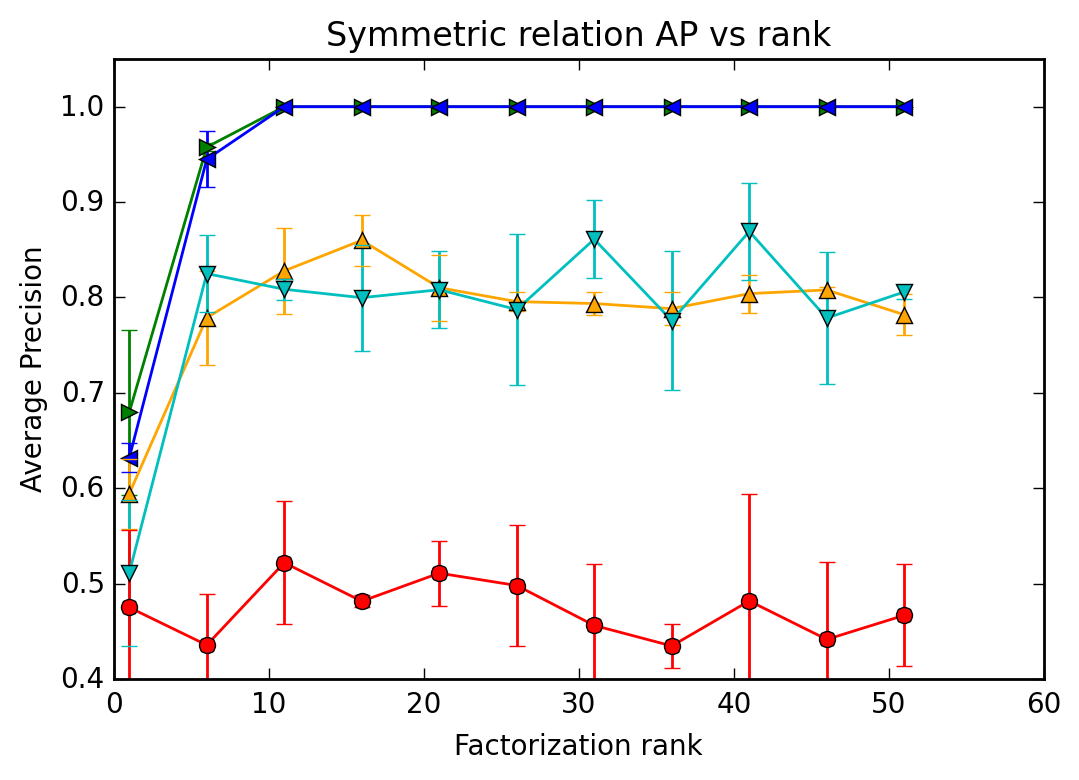
\includegraphics[width=0.40\textwidth]{symmetric_rel_ap_vs_rank.png}
	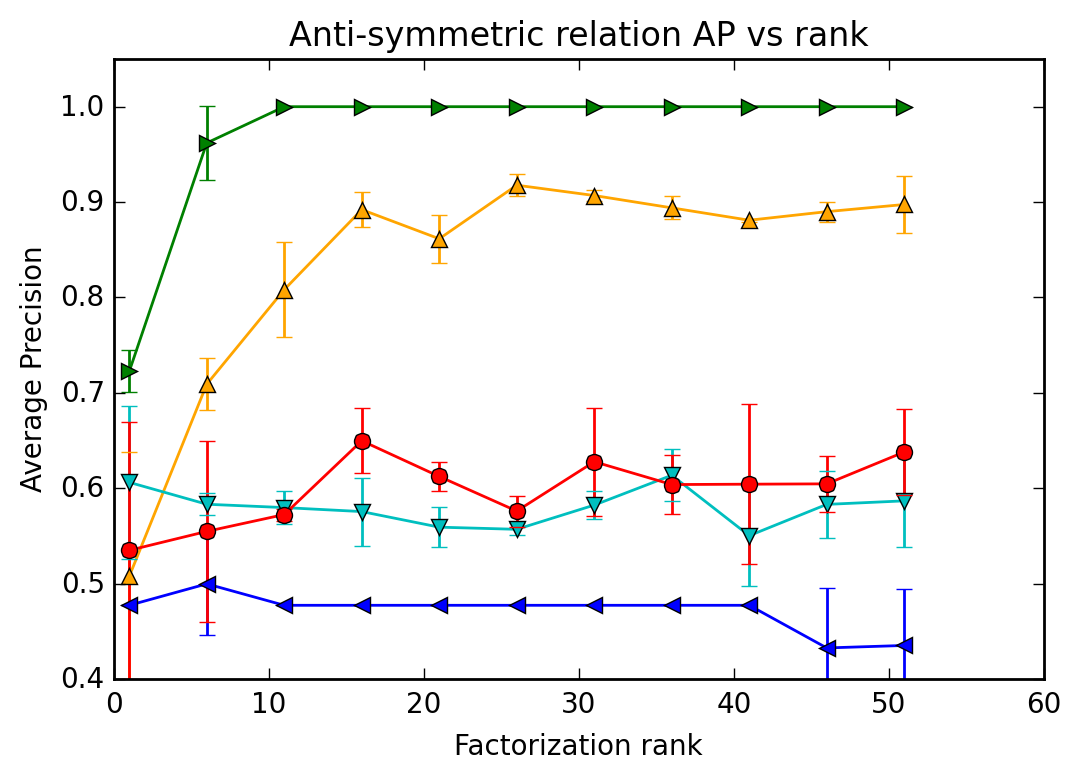
\includegraphics[width=0.40\textwidth]{antisymmetric_rel_ap_vs_rank.png} 
	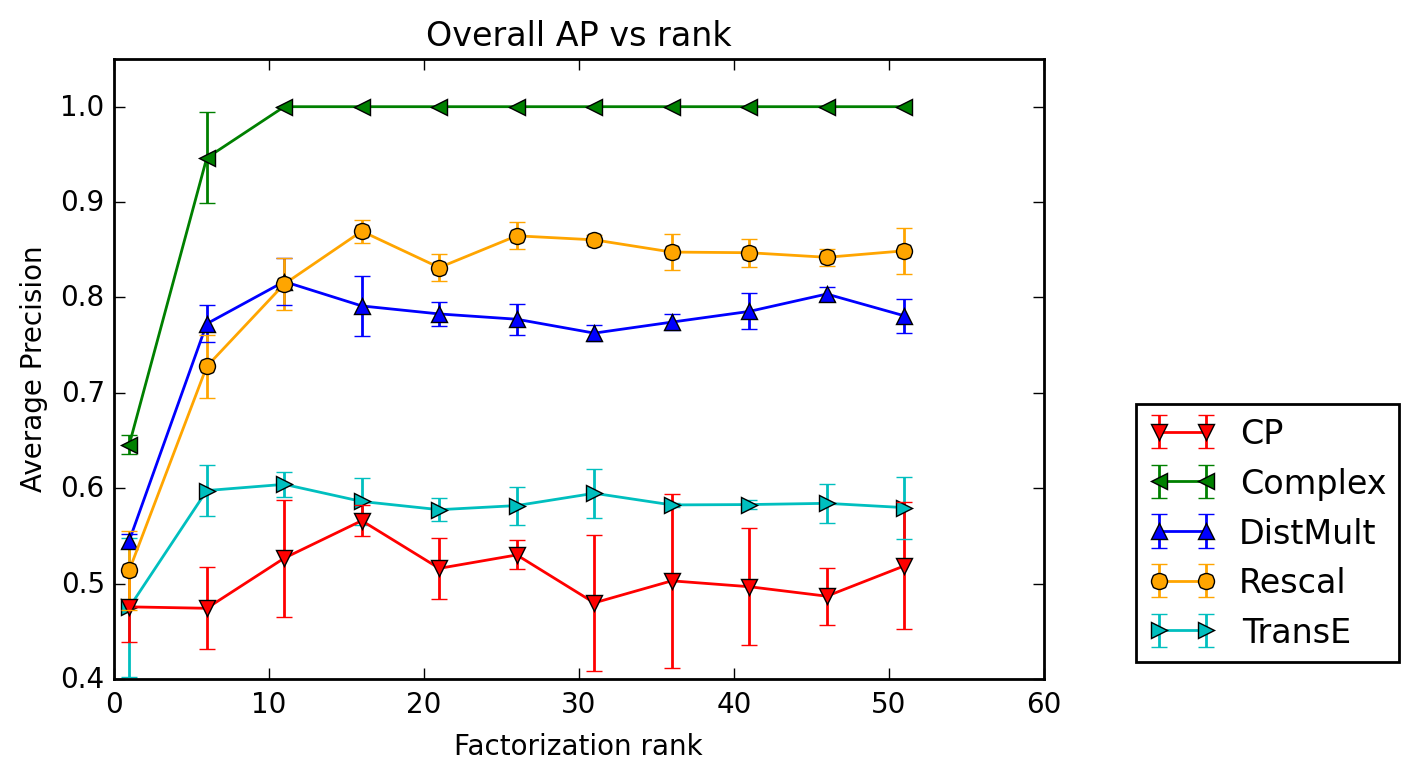
\includegraphics[width=0.51\textwidth]{overall_ap_vs_rank.png}
	%\vspace{-5mm}
	\caption{Average Precision (AP) for each factorization rank ranging from 1 to 50 for different state of the art models on the combined symmetry and antisymmetry experiment. Top-left: AP for the symmetric relation only. Top-right: AP for the antisymmetric relation only. Bottom: Overall AP.}
	\label{fig:exp_sym_antisym}
\end{figure*}

\subsection{Synthetic Task}

To assess the ability of our proposal to accurately model symmetry and antisymmetry, we randomly generated a KB of two relations and 30 entities. One relation is entirely symmetric, while the other is completely antisymmetric. This dataset corresponds to a $2 \times 30 \times 30$ tensor. Figure \ref{fig:symmetry_example} shows a part of this randomly generated tensor, with a symmetric slice and an antisymmetric slice, decomposed into training, validation and test sets. The diagonal is unobserved as it is not relevant in this experiment.

The train set contains 1392 observed triples, whereas the validation and test sets contain 174 triples each. Figure \ref{fig:exp_sym_antisym} shows the best cross-validated Average Precision (area under Precision-Recall curve) for different factorization models of ranks ranging up to 50. Models were trained using Stochastic Gradient Descent with mini-batches and AdaGrad for tuning the learning rate~\cite{duchi2011adaptive}, by minimizing the negative log-likelihood of the logistic model with $L^2$ regularization on the parameters $\Theta$ of the considered model:
\begin{equation}
    \min_{\Theta} \sum_{r(s,o) \in \Omega} \log( 1 + \exp(-\ObsTensor_{rso}\phi(s,r,o;\Theta))) + \lambda ||\Theta||^2_2\enspace.
\end{equation}
In our model, $\Theta$ corresponds to the embeddings $e_s,w_r,e_o \in \C^K$.
We describe the full algorithm in Appendix \ref{app:sgd}.

$\lambda$ is validated in $\{0.1, 0.03,$ $ 0.01, 0.003,$ $ 0.001, 0.0003,$ $ 0.00001, 0.0\}$. As expected, DistMult \cite{Yang2015} is not able to model antisymmetry and only predicts the symmetric relations correctly. Although TransE \cite{bordes2013translating} is not a symmetric model, it performs poorly in practice, particularly on the antisymmetric relation. 
RESCAL \cite{Nickel2011}, with its large number of parameters, quickly overfits as the rank grows. Canonical Polyadic (CP) decomposition \cite{hitchcock-sum-1927} fails on both relations as it has to push symmetric and antisymmetric patterns through the entity embeddings. Surprisingly, only our model succeeds on such simple data.

\begin{figure}
	\centering
	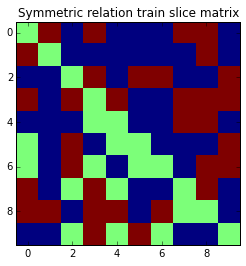
\includegraphics[width=0.32\linewidth]{exp_symmetry_train.png}
	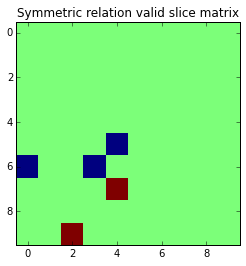
\includegraphics[width=0.32\linewidth]{exp_symmetry_valid.png}
	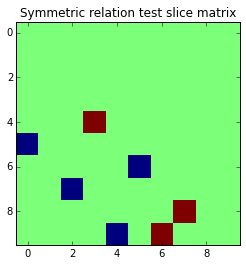
\includegraphics[width=0.32\linewidth]{exp_symmetry_test.png}
	
	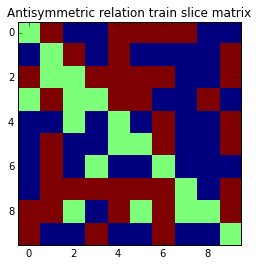
\includegraphics[width=0.32\linewidth]{exp_antisymmetric_train.png}
	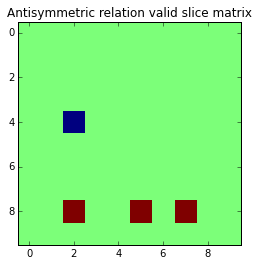
\includegraphics[width=0.32\linewidth]{exp_antisymmetric_valid.png}
	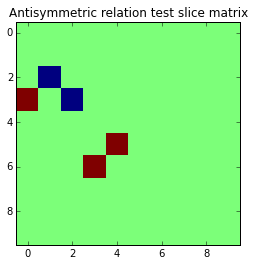
\includegraphics[width=0.32\linewidth]{exp_antisymmetric_test.png}

    \caption{Parts of the training, validation and test sets of the generated experiment with one symmetric and one antisymmetric relation. Red pixels are positive triples, blue are negatives, and green missing ones. Top: Plots of the symmetric slice (relation) for the 10 first entities. Bottom: Plots of the antisymmetric slice for the 10 first entities.}
	\label{fig:symmetry_example}
\end{figure}

%\begin{figure}[H]
%	\centering
%	\includegraphics[width=0.99\linewidth]{symmetry_ap_vs_rank.png}\\
%	\includegraphics[width=0.99\linewidth]{antisymmetry_ap_vs_rank.png}
%	\caption{Average Precision for each factorization rank ranging from 1 to 20 of each model on the symmetry and antisymmetry experiments.}
%	\label{fig:exp_symmetry}
%\end{figure}


%\begin{figure}[H]
%	\centering
%	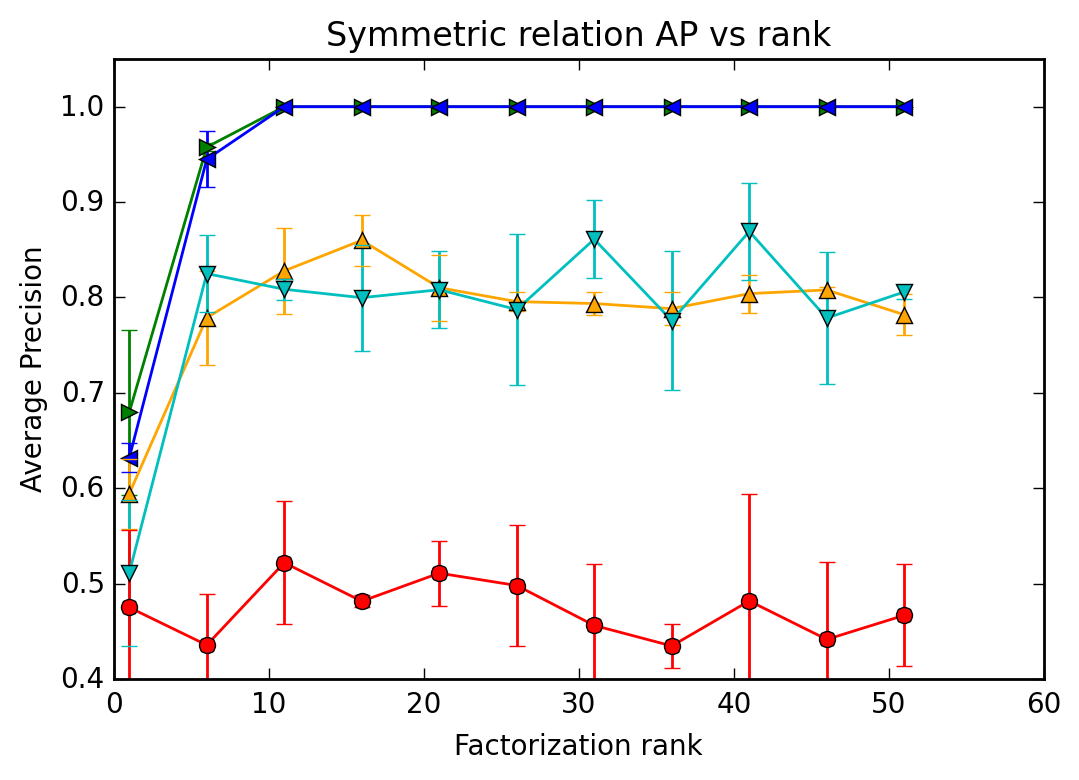
\includegraphics[width=0.49\linewidth]{symmetric_rel_ap_vs_rank.png}
%	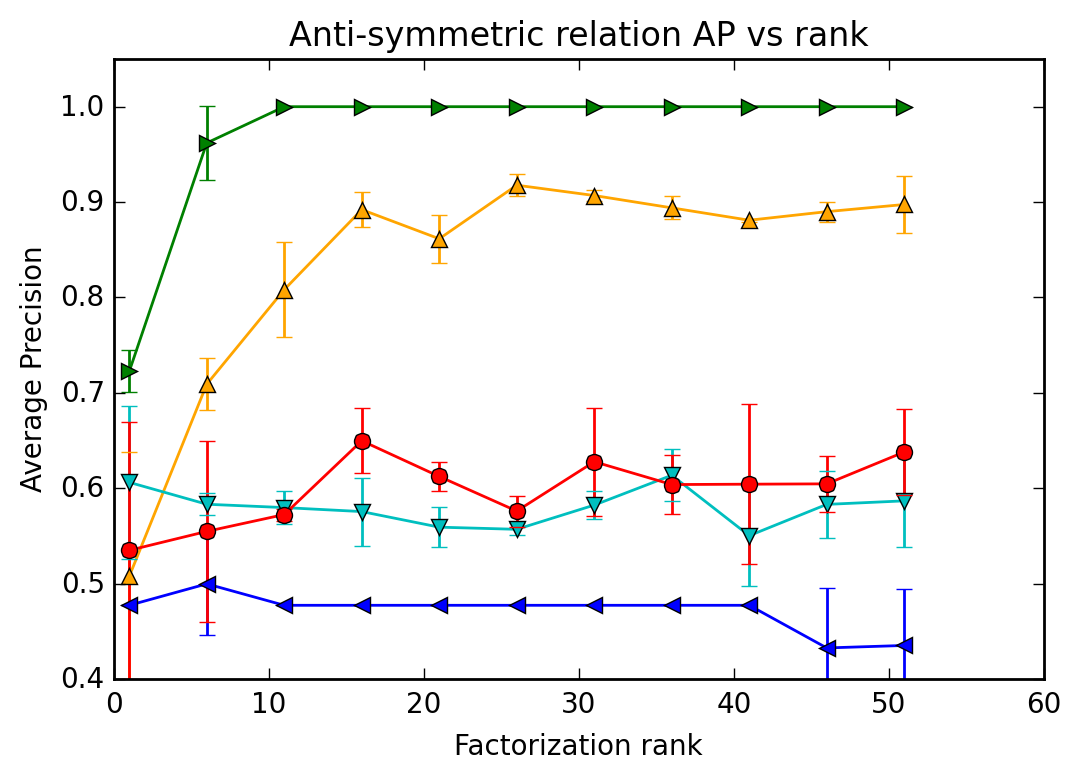
\includegraphics[width=0.49\linewidth]{antisymmetric_rel_ap_vs_rank.png} \\
%	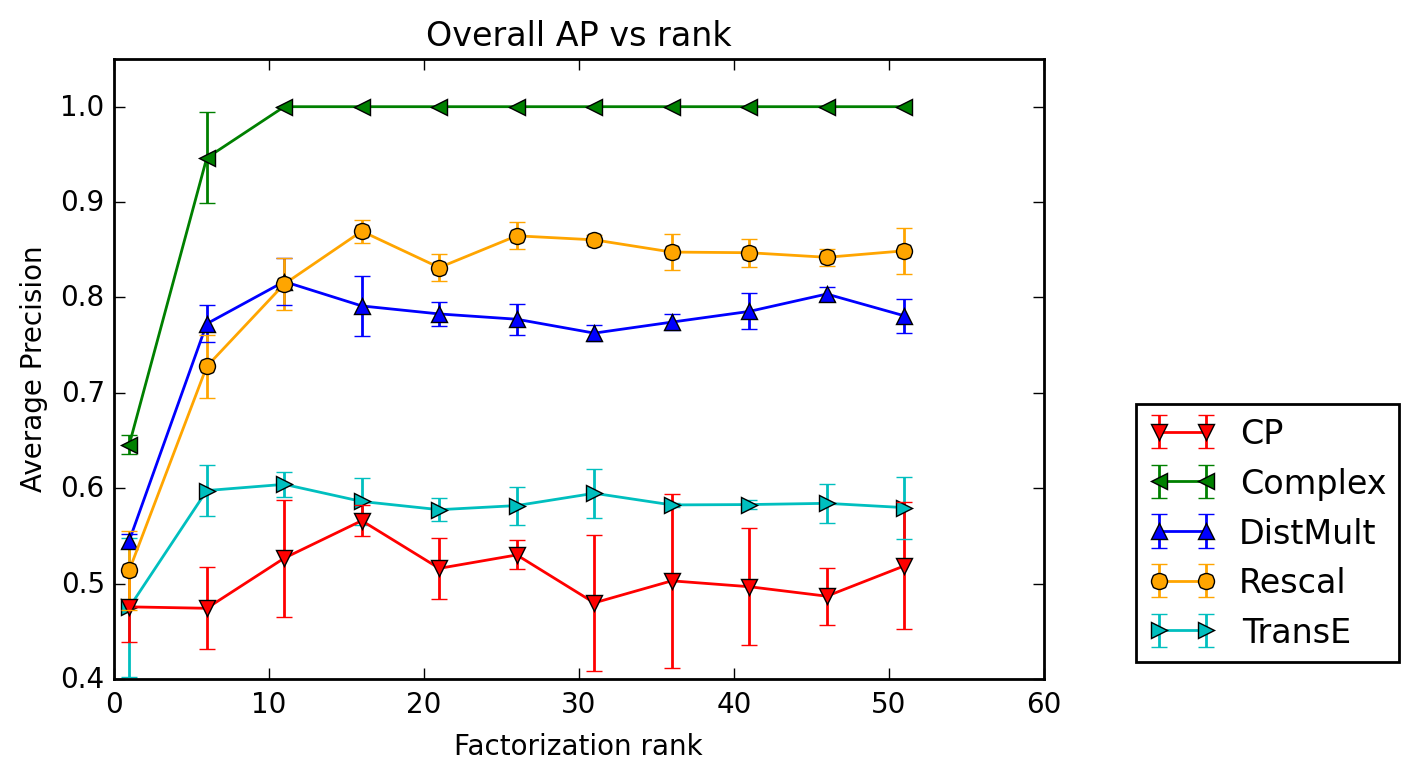
\includegraphics[width=0.65\linewidth]{overall_ap_vs_rank.png}
%	\caption{Average Precision (AP) for each factorization rank ranging from 1 to 50 for different state of the art models on the combined symmetry and antisymmetry experiment. Top-left: AP on the symmetric relation only. Top-right: AP the antisymmetric relation only. Bottom: Overall AP.}
%	\label{fig:exp_sym_antisym}
%\end{figure}



%%%%%%%%%%%%%%%%%%%%%%%%%%%%%%%%%%%%%%%%%%%%%%%%%%%%%%
%Have to put it here to make it appear on the right page
\begin{table*}[t]
    \centering
    \begin{tabular}{@{\extracolsep{8pt}}lllllllllll@{}}
        \toprule
        
         & \multicolumn{5}{c}{\textbf{WN18}} & \multicolumn{5}{c}{\textbf{FB15K}} \\ \cline{2-6} \cline{7-11}
         & \multicolumn{2}{c}{MRR} & \multicolumn{3}{c}{Hits at} & \multicolumn{2}{c}{MRR} & \multicolumn{3}{c}{Hits at} \\ \cline{2-3} \cline{4-6} \cline{7-8} \cline{9-11}
        
        Model & Filter & Raw & 1 & 3 & 10 & Filter & Raw & 1 & 3 & 10 \\ \hline
        
        CP & 0.075 & 0.058 & 0.049 & 0.080 & 0.125 & 0.326 & 0.152 & 0.219 & 0.376 & 0.532 \\
        TransE & 0.454 & 0.335 & 0.089 & 0.823 & 0.934 & 0.380 & 0.221 & 0.231 & 0.472 &  0.641 \\
        DistMult & 0.822 & 0.532 & 0.728 & 0.914 & 0.936 & 0.654 & \textbf{0.242} & 0.546 & 0.733   & 0.824 \\ 
        HolE* & 0.938 & \textbf{0.616} & 0.93 & \textbf{0.945} & \textbf{0.949} & 0.524 & 0.232 & 0.402 & 0.613 & 0.739\\ \hline
        ComplEx & \textbf{0.941} &  0.587 &  \textbf{0.936} &  \textbf{0.945} &  0.947 & \textbf{0.692} & \textbf{0.242} & \textbf{0.599} & \textbf{0.759}   & \textbf{0.840} \\
        
        \bottomrule
    \end{tabular}
    \caption{Filtered and Raw Mean Reciprocal Rank (MRR) for the models tested on the FB15K and WN18 datasets. Hits@m metrics are filtered. *Results reported from \cite{nickel_2016_holographic} for HolE model.}
    \label{tab:fb15k_wn18_res}
\end{table*}
%%%%%%%%%%%%%%%%%%%%%%%%%%%%%%%%%%%%%%%%%%%%%%%%%%%%%%%%%%%%%








\subsection{Datasets: FB15K and WN18}

%CV parameters + negative generation
\begin{table}[h]
    \centering
    \begin{tabular}{l|lll}
        Dataset & $|\EntitySpace|$ & $|\RelationSpace|$ & \#triples in Train/Valid/Test \\ \hline
        WN18 & 40,943 & 18 & 141,442 / 5,000 / 5,000 \\
        FB15K & 14,951 & 1,345 & 483,142 / 50,000 / 59,071 \\
    \end{tabular}
    \caption{Number of entities, relations, and observed triples in each split for the FB15K and WN18 datasets.}
    \label{tab:fb15k_wn18_meta}
\end{table}


We next evaluate the performance of our model on the FB15K and WN18 datasets. FB15K is a subset of \emph{Freebase}, a curated KB of general facts, whereas WN18 is a subset of \emph{Wordnet}, a database featuring lexical relations between words.  We use original training, validation and test set splits as provided by \citet{bordes2013translating}. Table \ref{tab:fb15k_wn18_meta} summarizes the metadata of the two datasets.



Both datasets contain only positive triples. As in \citet{bordes2013translating}, we generated negatives using the \emph{local closed world assumption}. That is, for a triple, we randomly change either the subject or the object at random, to form a negative example. 
%too, giving: $r(s',o), \ObsTensor_{rs'o} = -1$ or $r(s,o'), \ObsTensor_{rso'} = -1$, where $s',o' \in \setent$.
 This negative sampling is performed at runtime for each batch of training positive examples. 


For evaluation, we measure the quality of the ranking of each test triple among all possible subject and object substitutions
: $r(s',o)$ and $r(s,o')$, $\forall s', \forall o' \in \setent$.
 Mean Reciprocal Rank (MRR) and Hits at $m$ are the standard evaluation measures for these datasets and come in two flavours: raw and filtered \cite{bordes2013translating}. The filtered metrics are computed \emph{after} removing all the other positive observed triples that appear in either training, validation or test set from the ranking, whereas the raw metrics do not remove these. %before computing MRR and the ratio of appearance of $r(s,o)$ in the $n$ most probable triples (Hits at $n$), 
%In contrast, the raw metrics do not . 


Since ranking measures are used, previous studies generally preferred a pairwise ranking loss for the task \cite{bordes2013translating,nickel_2016_holographic}. We chose to use the negative log-likelihood of the logistic model, as it is a continuous surrogate of the sign-rank, and has been shown to learn compact representations for several important relations, especially for transitive relations~\cite{bouchard2015}. In preliminary work, we tried both losses, and indeed the log-likelihood yielded better results than the ranking loss (except with TransE), especially on FB15K.


We report both filtered and raw MRR, and filtered Hits at 1, 3 and 10 in Table \ref{tab:fb15k_wn18_res} for the evaluated models. Furthermore, we chose TransE, DistMult and HolE as baselines since they are the best performing models on those datasets to the best of our knowledge \cite{nickel_2016_holographic,Yang2015}. We also compare with the CP model to emphasize empirically the importance of learning unique embeddings for entities. 
For experimental fairness, we reimplemented these methods within the same framework as the ComplEx model, using theano~\cite{theano}. 
However, due to time constraints and the complexity of an efficient implementation of HolE, we record the original results for HolE as reported in \citet{nickel_2016_holographic}.
%However due to the complexity of the HolE model and time constraints, we couldn't re-implement it, we report results from \cite{nickel_2016_holographic} for this model.



\subsection{Results}


WN18 describes lexical and semantic hierarchies between concepts and contains many antisymmetric relations such as hypernymy, hyponymy, or being "part of". Indeed, the DistMult and TransE models are outperformed here by ComplEx and HolE, which are on par with respective filtered MRR scores of 0.941 and 0.938. %, thanks to their ability to model antisymmetry. 
Table \ref{tab:wn18_detailed_res} shows the filtered test set MRR for the models considered and each relation of WN18, confirming the advantage of our model on antisymmetric relations while losing nothing on the others. 2D projections of the relation embeddings provided in Appendix \ref{app:wn18_pca} visually corroborate the results.

\begin{table}
    \begin{tabular}{l|l@{\hspace{0.5em}}l@{}@{\hspace{0.5em}}l@{}}
        %\toprule
        
        Relation name & ComplEx & DistMult & TransE\\ \hline
        hypernym  & \textbf{0.953} & 0.791 & 0.446 \\
        hyponym  & \textbf{0.946} & 0.710 & 0.361 \\
        member\_meronym  & \textbf{0.921} & 0.704 & 0.418 \\
        member\_holonym  & \textbf{0.946} & 0.740 & 0.465 \\
        instance\_hypernym  & \textbf{0.965} & 0.943 & 0.961 \\
        instance\_hyponym  & \textbf{0.945} & 0.940 & 0.745 \\
        has\_part  & \textbf{0.933} & 0.753 & 0.426 \\
        part\_of  & \textbf{0.940} & 0.867 & 0.455 \\
        member\_of\_domain\_topic  & \textbf{0.924} & 0.914 & 0.861 \\
        synset\_domain\_topic\_of  & \textbf{0.930} & 0.919 & 0.917 \\
        member\_of\_domain\_usage  & \textbf{0.917} & \textbf{0.917} & 0.875 \\
        synset\_domain\_usage\_of  & \textbf{1.000} & \textbf{1.000} & \textbf{1.000} \\
        member\_of\_domain\_region  & \textbf{0.865} & 0.635 & \textbf{0.865} \\
        synset\_domain\_region\_of  & 0.919 & 0.888 & \textbf{0.986} \\
        derivationally\_related\_form  & \textbf{0.946} & 0.940 & 0.384 \\
        similar\_to  & \textbf{1.000} & \textbf{1.000} & 0.244 \\
        verb\_group  & \textbf{0.936} & 0.897 & 0.323 \\
        also\_see  & 0.603 & \textbf{0.607} & 0.279 \\

        %\bottomrule
    \end{tabular}
    \caption{Filtered Mean Reciprocal Rank (MRR) for the models tested on each relation of the Wordnet dataset (WN18).}
    \label{tab:wn18_detailed_res}
    
    \vspace{-5mm}
\end{table}

On FB15K, the gap is much more pronounced and the ComplEx model largely outperforms HolE, with a filtered MRR of 0.692 and 59.9\% of Hits at 1, compared to 0.524 and 40.2\% for HolE. We attribute this to the simplicity of our model and the different loss function. This is supported by the relatively small gap in MRR compared to DistMult (0.654); our model can in fact be interpreted as a complex number version of DistMult. 
%since our model can be seen as a complex numbers version of DistMult, and the DistMult scores are very close with 0.654 MRR. 
On both datasets, TransE and CP are largely left behind. This illustrates the power of the simple dot product in the first case, and the importance of learning unique entity embeddings in the second. CP performs poorly on WN18 due to the small number of \mbox{relations}, which magnifies this subject/object difference.



%\subsection{Experimental Details}
Reported results are given for the best set of hyper-parameters evaluated on the validation set for each model, after grid search on the following values: $\rank \in \{10,20,50,100,150,200\}$, $\lambda \in \{0.1, 0.03, 0.01, 0.003, 0.001, 0.0003,0.0\}$, $\alpha_0 \in \{1.0, 0.5, 0.2, 0.1, 0.05, 0.02, 0.01\}$,  $\eta \in \{1, 2, 5, 10\}$ with $\lambda$ the $L^2$ regularization parameter, $\alpha_0$ the initial learning rate (then tuned at runtime with AdaGrad), and $\eta$ the number of negatives generated per positive training triple. We also tried varying the batch size but this had no impact and we settled with 100 batches per epoch. Best ranks were generally 150 or 200, in both cases scores were always very close for all models. The number of negative samples per positive sample also had a large influence on the filtered MRR on FB15K (up to +0.08 improvement from 1 to 10 negatives), but not much on WN18. On both datasets regularization was important (up to +0.05 on filtered MRR between $\lambda=0$ and optimal one).
We found the initial learning rate to be very important on FB15K, while not so much on WN18. We think this may also explain the large gap of improvement our model provides on this dataset compared to previously published results -- as DistMult results are also better than those previously reported \cite{Yang2015} -- along with the use of the log-likelihood objective. It seems that in general AdaGrad is relatively insensitive to the initial learning rate, perhaps causing some overconfidence in its ability to tune the step size online and consequently leading to less efforts when selecting the initial step size.
%TransE results however are consistent \cite{nickel_2016_holographic,bordes2013translating}. 

Training was stopped using early stopping on the validation set filtered MRR, computed every 50 epochs with a maximum of 1000 epochs.

\subsection{Influence of Negative Samples}
We further investigated the influence of the number of negatives generated per positive training sample. In the previous experiment, due to computational limitations, the number of negatives per training sample, $\eta$, was validated among the possible numbers $\{1, 2, 5, 10\}$. We want to explore here whether increasing these numbers could lead to better results. To do so, we focused on FB15K, with the best validated $\lambda,\rank,\alpha_0$, obtained from the previous experiment. We then let $\eta$ vary in $\{1, 2, 5, 10, 20, 50, 100, 200\}$.

%is we couldn't extend our grid search beyond 10 negatives per train sample, since we also wanted to make sure that every model is treated fairly. However using GPU acceleration we ran our model on more on FB15K, using the best validated $\lambda,\rank,\alpha_0$ in the previous experiment, and then increasing $\eta \in \{20,50,100,200\}$. The results reported in Figure \ref{fig:neg_ratio} are hence lower bounds over what could yield higher number of generated positives, as the hyper-parameters have been validated with $\eta=\in\{1,2,5,10\}$.


Figure \ref{fig:neg_ratio} shows the influence of the number of generated negatives per positive training triple on the performance of our model on FB15K.
Generating more negatives clearly improves the results, with a filtered MRR of 0.737  with 100 negative triples (and 64.8\% of Hits@1), before decreasing again with 200 negatives. The model also converges with fewer epochs, which compensates partially for the additional training time per epoch, up to 50 negatives. It then grows linearly as the number of negatives increases, making 50 a good trade-off between accuracy and training time. %Due to computational limits, we couldn't run our grid-search with such high numbers of negatives, this is why reported results in Table \ref{tab:fb15k_wn18_res}  (up to 10 negatives) are lower than those. \Johans{This great result looks somehow insignificant between those discussions of hyperparameters, let's have it a bit more prominent?}


\begin{figure}[h]
	\centering
	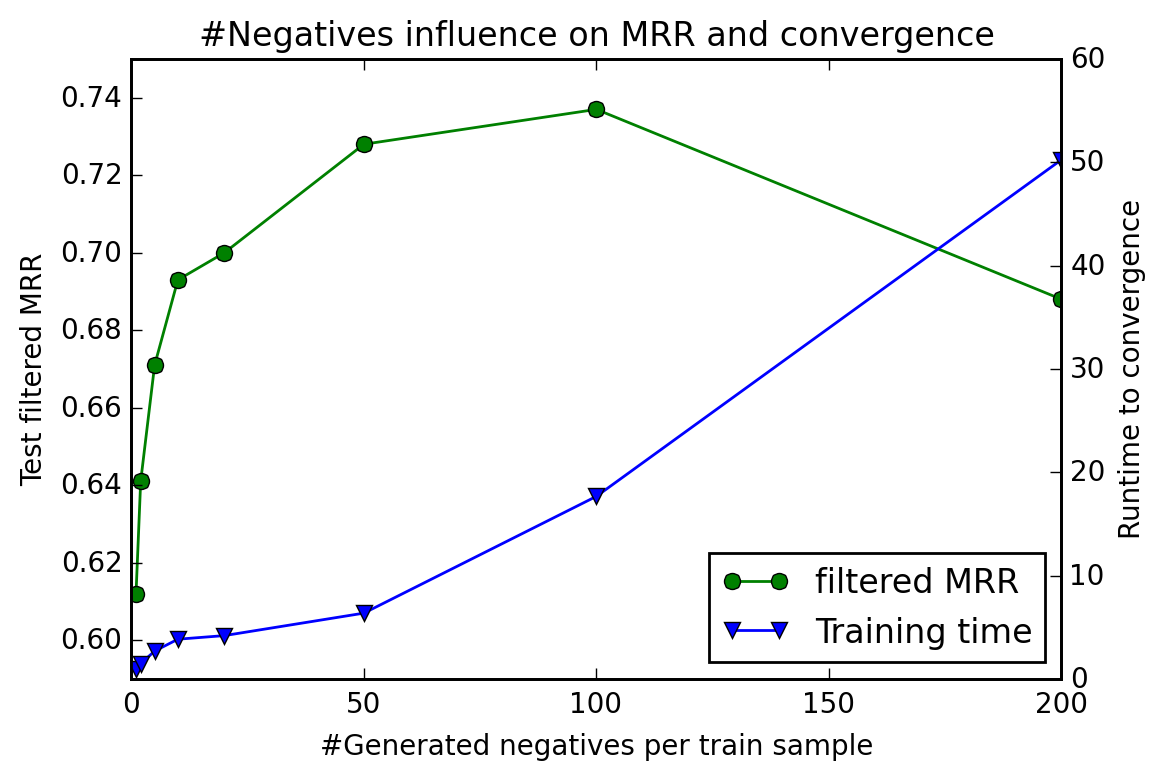
\includegraphics[width=0.99\linewidth]{neg_ratio_plot.png}
	
    \caption{Influence of the number of negative triples generated per positive training example on the filtered test MRR and on training time to convergence on FB15K for the ComplEx model with $\rank=200$, $\lambda=0.01$ and $\alpha_0=0.5$. Times are given relative to the training time with one negative triple generated per positive training sample ($=1$ on time scale).}
	\label{fig:neg_ratio}
	
\end{figure}


%\Seb{Somehow the negative data experiments don't fit that well into the story.It's not a big problem though. How about an analysis of the real and imaginary relation norms to back up the statement made earlier about these norms. }


%TODO: Write about the grid search values.
% ranks: [10,20,50,100,150,200]
%lmbdas: [0.1, 0.03, 0.01, 0.003, 0.001, 0.0003, 0.00001]
% alpha init: 1.0, 0.5, 0.2, 0.1, 0.05, 0.02, 0.01
% neg_ratio: 1, 2, 5, 10
% margins : 0.1, 0.5, 1.0, 2.0, + L2 and L1 distances for transE


%Initial learning rate very important for FB15K, not much for WN18
%negative_prop increase a lot MRR on FB15K ( up to 5-6 points? or just not converged and just accelerate? -> Nope, actually gets up to 5 points higher (63 to 68), and too much decrease.), not on WN18
%Lambda (best around 0.01) important, about 5 points with too low lambda, much more with too high one
%Best ranks generally between 100 and 200
%Batch size not important, used 100 batches
%Early stopping on validation filtered MRR every 100 its


%About overconfidence in adagrad, depends on dataset (i.e FB important (otherwise loss stall) WN not)

%local closed world assumption and negative generation, and plot by nb of negatives






%\Johans{Can't present results that look like tuned on test set.}








\section{Related Work}
In the early age of spectral theory in linear algebra, complex numbers were not used 
for matrix factorization and mathematicians mostly focused on bi-linear forms~\cite{beltrami1873sulle}. 
The eigen-decomposition in the complex domain as taught today in linear algebra courses 
came 40 years later~\cite{autonne1915}. Similarly, most of the existing approaches for tensor 
factorization were based on decompositions in the real domain, such as the Canonical Polyadic (CP) decomposition~\cite{hitchcock-sum-1927}. These methods are very effective in many applications 
that use different modes of the tensor for different types of entities.
But in the link prediction problem, antisymmetry of relations was quickly seen as 
a problem and asymmetric extensions of tensors were studied, mostly by either
considering independent embeddings~\cite{sutskever2009} or considering relations as
matrices instead of vectors in the RESCAL model~\cite{Nickel2011}. 
Direct extensions were based on uni-,bi- and trigram latent factors for triple data, as well as a low-rank relation matrix~\cite{Jenatton2012}. 

Pairwise interaction models were also considered to improve prediction performances. For example, the Universal Schema approach~\cite{riedel_2013_univschema} factorizes a 2D unfolding of the tensor (a matrix of entity pairs vs. relations) while \citet{Welbl2016} extend this also to other pairs.

%where each row corresponds to an possible pair of entity. 
% It had been extended with a joint tensor factorization \cite{Singh2015}, and to take into account logical prior on the data \cite{Rocktaschel2015}. 
In the Neural Tensor Network (NTN) model, \citet{socher2013reasoning} combine linear transformations and multiple bilinear forms of subject and object embeddings to jointly feed them into a nonlinear neural layer. Its non-linearity and multiple ways of including interactions between embeddings gives it an advantage in expressiveness over models with simpler scoring function like DistMult or RESCAL. As a downside, its very large number of parameters can make the NTN model harder to train and overfit more easily.

The original multi-linear DistMult model is symmetric in subject and object for every relation ~\cite{Yang2015} and achieves good performance, presumably due to its simplicity.
%A surprising finding is that the original multi-linear model (symmetric in object and subject for every relation), such as the DistMult model~\cite{Yang2015}, still leads to good performance, thanks to its simplicity.
%\Seb{So in these papers they have used it with more data than other models?}
The TransE model from \citet{bordes2013translating} also embeds entities and relations in the same space and imposes a geometrical structural bias into the model: the subject entity vector should be close to the object entity vector once translated by the relation vector.
%\Johans{Not sure, but I thought the TransE scoring function is asymmetric in the entities}
% Injecting logical background in factorization model \cite{Rocktaschel2015} 


A recent novel way to handle antisymmetry is via the Holographic Embeddings (HolE) model by ~\cite{nickel_2016_holographic}. In HolE the circular correlation is used for combining entity embeddings, measuring the covariance between embeddings at different dimension shifts. This generally suggests that other composition functions than the classical tensor product can be  helpful as they allow for a richer interaction of embeddings. However, the asymmetry in the composition function in HolE stems from the asymmetry of circular correlation, an $\mathcal{O}(n log(n))$ operation, whereas ours is inherited from the complex inner product, in $\mathcal{O}(n)$.

%The use of complex numbers have already been considered for the link prediction problem, using graph theory based methods \cite{kunnegis,feng}.




% More recently, the HolE model \cite{nickel_2016_holographic} uses the same embeddings as DistMult, but combines them using circular correlation instead of a dot product. This yields state of the art performances on both FB15K and WordNet18 datasets.


% Combined matrix and tensor factorization \cite{Singh2015}
% Typed tensor factorization (TRESCAL) \cite{Chang2014}
%Other 
%Distant supervision for relation extraction without labeled data \cite{Mintz2009}
%Multi-instance multi-label learning for relation extraction \cite{Surdeanu2012}
%RESCAL, ARE, HOLE, Review \cite{Nickel2011,Nickel2014,nickel_2016_holographic,nickel_2016_review} 

% DistMult{Toutanova2015}
  


% Early models: Learning structured embeddings of knowledge bases \cite{Bordes2011}



% \cite{Nickel2011} proposed a major improvement over the CP decomposition, by unifying the subject and object entities latent factors $\eemb \in \R^{\Ne \times \rank} $ and learning one embedding matrix per relation instead of one vector $\Remb_r \in \R^{\Nr \times \rank} $, giving the RESCAL model: $ P(\sampval) = \sigma(( \eemb_s \times \Remb_r ) \cdot \eemb_r) $. When $\sigma(x)=x$, the squared loss is minimized, however in general the logistic loss $\sigma(x)= 1 / (1 + e^{-x})$ is preferred and known to yield better generalizations \cite{bouchard2015}.

% Many models derive from RESCAL, \cite{Jenatton2012} clustered the relation matrix embeddings together and added bias terms over pairs of entities/relations. TRESCAL \cite{Chang2014} integrates the information about the types of the entities in its RESCAL factorization. ARE model \cite{Nickel2014} extends by adding a linear term over observable patterns in the data. \cite{socher2013reasoning} proposes a generalization of RESCAL where relations have latent tensors instead of matrices, and adds a linear term over the entities embeddings and a bias, the final score is a linear combination of the sum of all those terms. The DistMult model simplifies RESCAL by going back to vectors embeddings for relations, while keeping shared embeddings for subject and object entities: $ P(\sampval) = \sigma(( \remb_r \cdot (\eemb_s \odot \eemb_r)  ) $\footnote{$\odot$ stands for the Hadamard product, i.e. the element-wise product between two vectors/matrices/tensors of the same dimensions.}. While the model lose it's capacity to model asymetric relations, it's simplicity gives it an advantage \cite{Yang2015,Toutanova2015}.

% \cite{Bordes2011,Bordes2014} learns 2 embedding vectors for each relations, one combined with the subject entity vector and the other with the object vector, optionally adding latent intermediate parameters to combine the intermediate scores. Eventually, simplicity had it again with the TransE model \cite{Bordes2014a}. It models relations as translations in the embedding space, from the subject embedding to the object embedding, minimizing a distance between the translated subject and the object : $d(\mathbf{s}_s+\mathbf{r}_r,\mathbf{o}_o)$, $d$ being either $L_1$ or $L^2$ norm.

% In this paper, we first build on the Universal Schema model, by using complex numbers to factorize the entiy-pairs/relations matrix. Then we extend the Hermitian product to 3-way factorization, in a similar way to DistMult model, but restoring modelling of symmetric and antisymmetric relations throught the use of the Hermitian product.







\section{Conclusion}

We described a simple approach to matrix and tensor factorization for link prediction data that uses vectors with complex values and retains the mathematical definition of the dot product. 
The class of normal matrices is a natural fit for binary relations, and using the real part allows for efficient approximation of any learnable relation. Results on standard benchmarks show that no more modifications are needed to improve over the state-of-the-art. 


%This leads us to characterize the class of matrices that can efficiently be approximated by the model, namely low-rank normal matrices, and showed in  that no more modifications are needed to improve over the state-of-the-art. 

There are several directions in which this work can be extended. An obvious one is to merge our approach with known extensions to tensor factorization in order to further improve predictive performance. For example, the use of pairwise embeddings together with complex numbers might lead to improved results in many situations that involve non-compositionality. %, i.e. pairs of entities that often appear together. 
Another direction would be to develop a more intelligent negative sampling procedure, to generate more informative negatives with respect to the positive sample from which they have been sampled. It would reduce the number of negatives required to reach good performance, thus accelerating training time.

Also, if we were to use complex embeddings every time a model includes a dot product, e.g. in deep neural networks, would it lead to a similar systematic improvement? 
%In fact, matrix and vector products are the main operations, together with component-wise non-linearities.

%\section*{Reproducibility}
%Code is currently under clearance review and will be available at: \url{https://github.com/ttrouill/complex}.



















%\begin{figure}[ht]
%\vskip 0.2in
%\begin{center}
%\centerline{\includegraphics[width=\columnwidth]{icml_numpapers}}
%\caption{Historical locations and number of accepted papers for International
%  Machine Learning Conferences (ICML 1993 -- ICML 2008) and
%  International Workshops on Machine Learning (ML 1988 -- ML
%  1992). At the time this figure was produced, the number of
%  accepted papers for ICML 2008 was unknown and instead estimated.}
%\label{icml-historical}
%\end{center}
%\vskip -0.2in
%\end{figure} 



\section*{Acknowledgements} 
This work was supported in part by the Paul
Allen Foundation through an Allen Distinguished
Investigator grant and in part by a Google Focused Research Award.

\bibliography{complex_bib,nonauto_bib}
\bibliographystyle{icml2016}






\clearpage



%\subsection{Symmetric/Skew-symmetric decomposition}
%Another way to view the decomposition into 
%the sum of a symmetric and skew-symmetric matrix:

%\begin{eqnarray}
%M &=& \underbrace{
%\frac 12 (M + \bar M\transp)
%}_{=S\ \mathrm{symmetric}}
%+ \underbrace{
%\frac 12 (M - \bar M\transp)
%}_{=A\ \mathrm{skew-symmetric}}
%\\
%&=& \bar{U}' D' (U')\transp + {\bar{U}'' (\i D'') (U'')\transp}
%\end{eqnarray}

%Factorization Machines \cite{Rendle2010, Rendle2013} allow for an efficient and generic way of incorporating higher-order interactions into a regression model. Utilising both pairwise embeddings and interactions thereof provided by the Factorization Machine, we not only use embeddings for pairs, but also their interactions inside the triple.
%In contrast, our work utilises embeddings for \emph{every} possible pair in the RDF 3-tuple. Letting pairs interact with one another allows to capture ternary interactions between both entities and the relation, something that \cite{Bordes2014a} already found to be useful in link prediction.
%[[[impose a low-rank constraint on the higher-order interactions of polynomial (mostly quadratic) regression. This allows for incorporating complex interactions into the prediction model, while not giving up on scalability. ]]]



\appendix


\section{SGD algorithm}
\label{app:sgd}
We describe the algorithm to learn the ComplEx model with Stochastic Gradient Descent using only real-valued vectors.

Let us rewrite equation \ref{eqn:sesquilinear-dot}, by denoting
the real part of embeddings with primes and the imaginary part with double primes: 
$e'_i = \real(e_i)$, $e''_i = \imag(e_i)$, $w'_r = \real(w_r)$, $w''_r = \imag(w_r)$.
The set of parameters is $\Theta=\{e'_i,e''_i,w'_r,w''_r; \forall
i \in \setent, \forall r \in \setrel \}$,
and the scoring function involves only real vectors:

\begin{eqnarray}
\phi(r,s,o;\Theta) &=& \left<w'_r,e'_s, e'_o\right>+ \left<w'_r,e''_s, e''_o\right> \notag\\
    &&+ \left<w''_r, e'_s, e''_o\right> - \left<w''_r,e''_s, e'_o\right>\notag
\end{eqnarray}

where each entity and each relation has two real embeddings. 


Gradients are now easy to write:


\begin{eqnarray}
\label{gradients}
\grad_{e'_s} \phi(r,s,o;\Theta) &=& (w'_r \odot e'_o) + (w''_r \odot e''_o)\notag\\
\grad_{e''_s} \phi(r,s,o;\Theta) &=& (w'_r \odot e''_o) - (w''_r \odot e'_o)\notag\\
\grad_{e'_o} \phi(r,s,o;\Theta) &=& (w'_r \odot e'_s) - (w''_r \odot e''_s)\notag\\
\grad_{e''_o} \phi(r,s,o;\Theta) &=& (w'_r \odot e''_s) + (w''_r \odot e'_s)\notag\\
\grad_{w'_r} \phi(r,s,o;\Theta) &=& (e'_s \odot e'_o) + (e''_s \odot e''_o)\notag\\
\grad_{w''_r} \phi(r,s,o;\Theta) &=& (e'_s \odot e''_o) - (e''_s \odot e'_o)\notag
\end{eqnarray}

where $\odot$ is the element-wise (Hadamard) product.


As stated in equation \ref{observation-model} we use the sigmoid link function, and minimize the $L^2$-regularized negative log-likelihood:

\begin{eqnarray}
    \gamma(\Omega;\Theta) &=&
    \sum_{r(s,o) \in \Omega} \log( 1 + \exp(-\ObsTensor_{rso}\phi(s,r,o;\Theta)))\notag\\
    &&+ \lambda ||\Theta||^2_2\enspace.\notag
\end{eqnarray}

To handle regularization, note that the squared $L^2$-norm of a complex vector $v=v'+iv''$
is the sum of the squared modulus of each entry:

\begin{eqnarray}
||v||^2_2 &=& \sum_j \sqrt{v_j^{\prime2} + v_j^{\prime\prime2}}^2\notag\\
&=& \sum_j v_j^{\prime2} + \sum_j  v_j^{\prime\prime2}\notag\\
&=& ||v'||^2_2 +  ||v''||^2_2\notag
\end{eqnarray}

which is actually the sum of the $L^2$-norms of the vectors of the real and imaginary parts.

We can finally write the gradient of $\gamma$ with respect to a \emph{real} embedding $v$ for
one triple $r(s,o)$:


\begin{eqnarray}
    \grad_v \gamma(\{r(s,o)\};\Theta) &=& -\ObsTensor_{rso}\phi(s,r,o;\Theta) \sigma(\grad_v \phi(r,s,o;\Theta))\notag\\
    &&+ 2\lambda v\notag
\end{eqnarray}

where $\sigma(x) = \frac{1}{1+\mathrm{e}^{-x}}$ is the sigmoid function.

Algorithm \ref{SGDC} describes SGD for this formulation of the
scoring function.
When $\Omega$ contains only positive triples,
we generate $\eta$ negatives per positive train triple, by corrupting
either the subject or the object of the positive triple, as 
described in \citet{bordes2013translating}.


\begin{algorithm}[t]
\caption{SGD for the ComplEx model}
\label{SGDC}
\begin{algorithmic}
\INPUT Training set $\Omega$, Validation set $\Omega_v$, learning rate $\alpha$, embedding dim. $k$, regularization factor $\lambda$, negative ratio $\eta$, batch size $b$, max iter $m$, early stopping $s$.
\STATE $e'_i \gets \randn(k)$, $e''_i \gets \randn(k)$ for each $i \in \mathcal{E}$
\STATE $w'_i \gets \randn(k)$, $w''_i \gets \randn(k)$ for each $i \in \mathcal{R}$
\FOR{$i=1,\cdots,m$}
    \FOR {$j=1..|\Omega|/b$}
        \STATE $\Omega_b \gets$ sample$(\Omega,b,\eta)$
        \STATE Update embeddings w.r.t.:\\
        $\quad\quad\sum_{r(s,o) \in \Omega_b} \grad \gamma(\{r(s,o)\};\Theta)$
        \STATE Update learning rate $\alpha$ using Adagrad
    \ENDFOR
    \IF{$i \mod s = 0$}
        \STATE \textbf{break} if filteredMRR or AP on $\Omega_v$ decreased
    \ENDIF
\ENDFOR
\end{algorithmic}
\end{algorithm}



\section{WN18 embeddings visualization}
\label{app:wn18_pca}


\begin{figure*}[!ht]%{{\extracolsep{8pt}}}
	\centering
	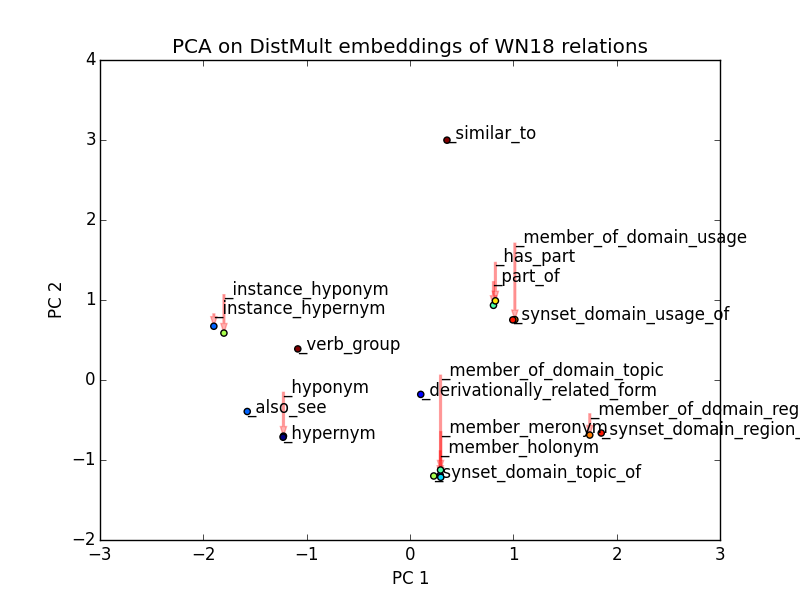
\includegraphics[width=0.49\textwidth]{distmult_pca_12.png}
	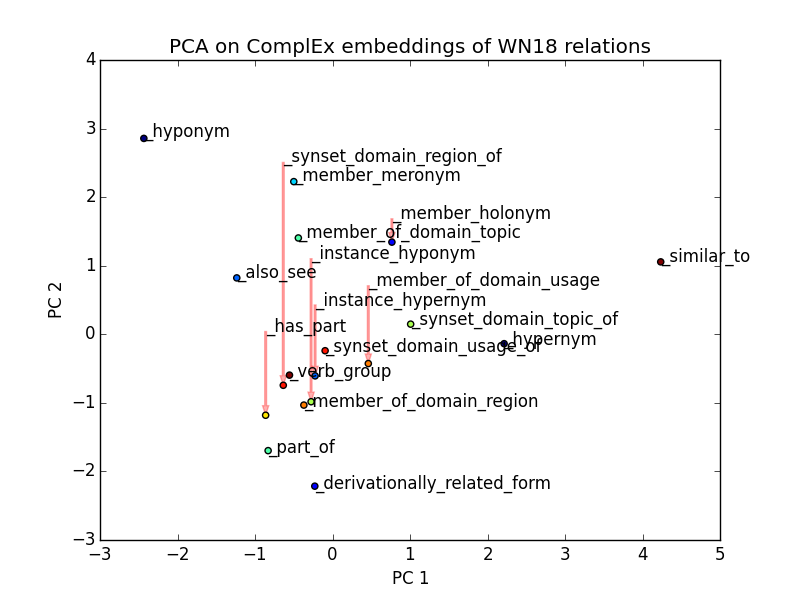
\includegraphics[width=0.49\textwidth]{complex_pca_12.png}
	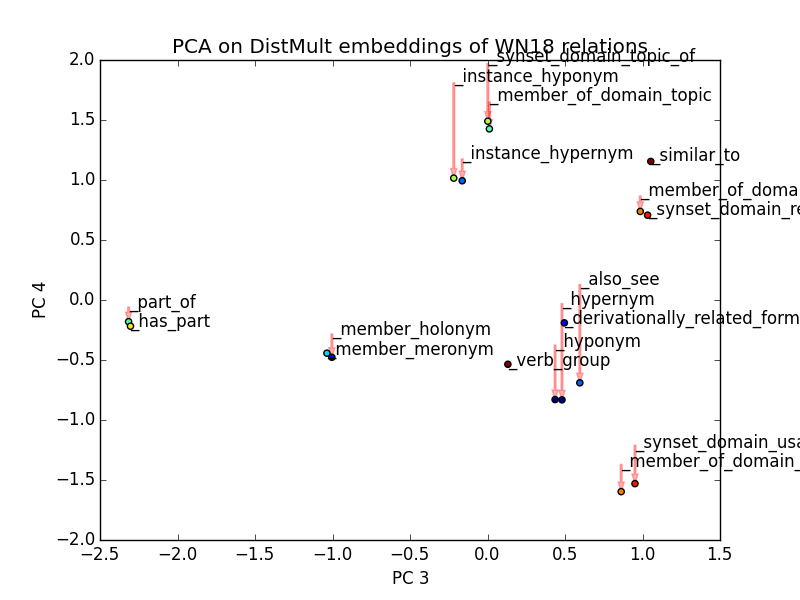
\includegraphics[width=0.49\textwidth]{distmult_pca_34.png}
	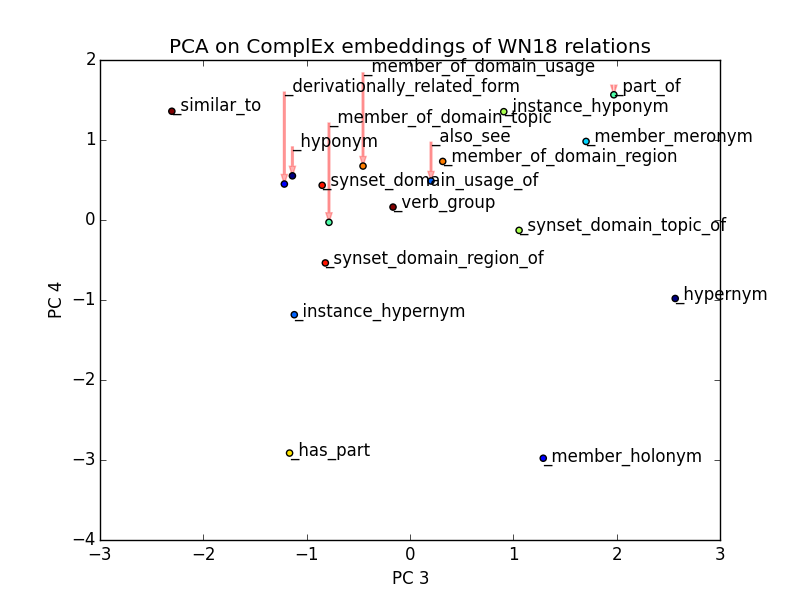
\includegraphics[width=0.49\textwidth]{complex_pca_34.png}
	\vspace{-5mm}
	\caption{Plots of the first and second (Top), third and fourth (Bottom) components of the WN18 relations embeddings using PCA. Left: DistMult embeddings. Right: ComplEx embeddings. Opposite
	relations are clustered together by DistMult while correctly separated by ComplEx.}
	\label{fig:pca}
\end{figure*}

We used principal component analysis (PCA) to visualize embeddings of the relations 
of the wordnet dataset (WN18). We plotted the four first components of the best DistMult
and ComplEx model's embeddings in Figure \ref{fig:pca}. For the ComplEx model, we simply concatenated
the real and imaginary parts of each embedding. 

Most of WN18 relations describe hierarchies, and are thus antisymmetric.
Each of these hierarchic relations has its inverse relation in the dataset. For example: \texttt{hypernym} / \texttt{hyponym},
\texttt{part\_of} / \texttt{has\_part}, \texttt{synset\_domain\_topic\_of} / \texttt{member\_of\_domain\_topic}.
Since DistMult is unable to model antisymmetry, it will correctly represent the nature
of each pair of opposite relations, but not the direction of the relations.
Loosely speaking, in the \texttt{hypernym} / \texttt{hyponym} pair the nature is 
sharing semantics,
and the direction is that one entity generalizes the semantics of the other. 
This makes DistMult reprensenting the opposite relations with very close embeddings,
as Figure \ref{fig:pca} shows. It is especially striking for the third and
fourth principal component (bottom-left). Conversely, ComplEx manages to oppose spatially
the opposite relations.




\end{document} 
